\documentclass[../report.tex]{subfiles}
\begin{document}	
	
\chapter{State of the art}
To understand the working principles of \gls{pr} it is important to look into the basic concepts of waveguides and the mathematics behind the propagation of \gls{em} waves. It is also necessary to understand tuning of optical waveguides using different mechanisms to achieve optical \gls{pr}. Finally, the integrated \gls{pr}s found in the recent literature and their underlying concepts are discussed. 

	\section{Optical waveguide theory}
Light can travel through dielectric waveguide. To comprehend the situation we need to look at the physical properties of light and waveguides. The basic understanding of Maxwell's equations is required. Maxwell combined the electric and magnetic fields in a wave equation. Since we need a formal definition of the different \gls{sop}, described using Jones calculus. Moreover, the rotation from one \gls{sop} to another, can be defined formally on the Poincaré sphere. 
		
		\subsection{Maxwell's equations}
Wave is a disturbance that propagates through a medium. Waves transfer both energy and momentum, without transferring any mass. \gls{em} radiation is the radiant energy released by varying \gls{em} field in the form of \gls{tem} waves. Light wave is \gls{em} radiation at very high frequency. The frequency of visible light falls in between IR and UV \gls{em} wave.
\begin{figure}[h]
	\centering
	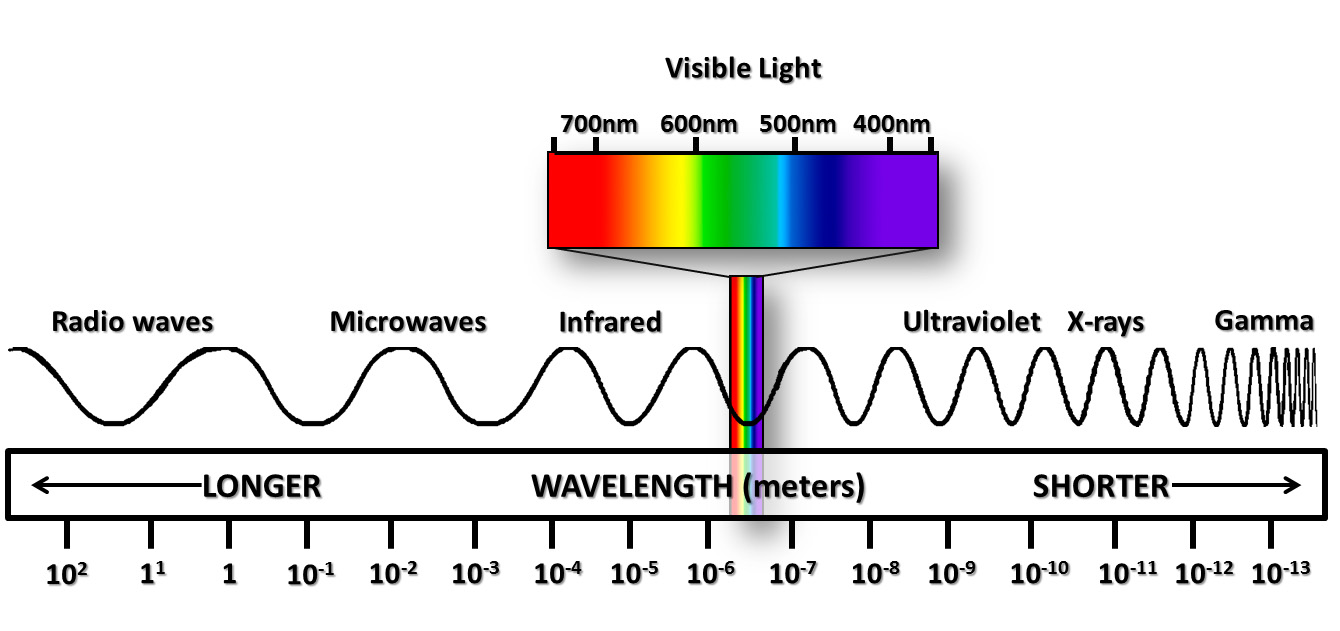
\includegraphics[width=0.75\textwidth]{2-light-spectrum}
	\caption{The \gls{em} wave spectrum}
	\label{fig:2_light_spectrum}
\end{figure}
James Clerk Maxwell discovered that he could combine four simple equations, which had been previously discovered, along with a slight modification to describe self-propagating waves of oscillating electric and magnetic fields \cite{waveparticle_2016}. The understanding of propagating of light waves using Maxwell's equations in a dielectric medium, is the key to the construction of waveguides. Maxwell’s equations relate the electric field $E$ (V/m), magnetic field $H$ (A/m), charge density $\rho$ (C/m3), and current density $J$ (A/cm2).
\begin{itemize}	
	\item \textbf{Maxwell's first equation (Gauss' Law)}: The net electric flux through any closed surface is equal to $\frac{1}{\epsilon_m}$ times the charge density within that closed surface.
	\begin{equation}\label{eq:max1_1}
	\nabla.E = \frac{\rho}{\epsilon_m}	
	\end{equation}
	where $\epsilon_m$ the permittivity of the medium, and del operator, $\nabla$, is given by:
	\begin{equation}\label{eq:max1_2}
	\nabla = \left(\frac{\partial i}{\partial x},\frac{\partial j}{\partial y},\frac{\partial k}{\partial z}\right)
	\end{equation}
	where i, j and k are unit vectors in the x, y and z directions respectively.
	
	\item \textbf{Maxwell's second equation (Gauss' Law for magnetic field)}: The net magnetic flux through a closed surface is always zero since magnetic monopoles do not exist.
	\begin{equation}\label{eq:max1_3}
	\nabla.H = 0	
	\end{equation}
	
	\item \textbf{Maxwell's third equation (Faraday's law)}: Induced electric field around a closed path is equal to the negative of the time rate of change of magnetic flux enclosed by the path.
	\begin{equation}\label{eq:max1_4}
	\nabla\times E = -\mu_m\frac{\partial H}{\partial t}
	\end{equation}
	where $\mu_m$ is the magnetic permeability of the medium.

	\item \textbf{Maxwell's fourth equation (Modification of Ampere's law)}:  The fourth equation states that magnetic fields can be generated in two ways: by electric current (this was the original “Ampere's law”) and by changing electric fields (this was “Maxwell's addition”) \cite{wiki_maxwells_2016}.
	\begin{equation}\label{eq:max1_5}
	\nabla\times H =  J + \epsilon_m\frac{\partial E}{\partial t}	
	\end{equation}
	where $\epsilon_m$ is the electric permittivity of the medium.	
\end{itemize}

\noindent These equations combine into the following wave equation
\begin{equation}\label{eq:wave_eq}
\nabla^2 E -  \mu_m\epsilon_m\frac{\partial^2 E}{\partial t^2} = \mu_m\frac{\partial J}{\partial t} + \frac{\nabla\rho}{\epsilon_m},	
\end{equation}
using the curl of curl identity operation given by 
\begin{equation}\label{eq:curl_of_curl}
\nabla^2 E = \nabla(\nabla.E) - \nabla\times(\nabla\times E).
\end{equation}
A general solution to the equation \ref{eq:wave_eq} in free space, in absence of charge is
\begin{equation}\label{eq:wave_sol_electric}
\overrightarrow{E}(z,t)=E_{0}(x,y)e^{i\left(\omega t \pm k_{0}z\right)},
\end{equation}
where $z$ is direction of propagation of wave in Cartesian coordinates, phase, $\phi$ = $\omega t \pm k_{0}z$ and wave vector propagation constant, $k_0$ = $\dfrac {\partial \phi } {\partial t}$ = $\dfrac {2\pi } {\lambda }$, in the direction of propagation of the wave. The propagation constant in medium varies according to $n_{eff}$, the effective \gls{ri} of the medium and is given by 
\begin{equation}\label{eq:propagation_const_med_val}
k = n_{eff}k_0,
\end{equation}
where
\begin{equation}\label{eq:ri_med_val}
n_{eff} = \sqrt {\varepsilon _{m}\mu _{m}}.
\end{equation}
Similar calculations for the magnetic field, $H$ in free space yields, 		
\begin{equation}\label{eq:wave_sol_magnetic}
\overrightarrow{H}(z,t)=H_{0}(x,y)e^{i\left(\omega t \pm k_{0}z\right)}
\end{equation}

\noindent In the Fig. \ref{fig:2_em_wave} the electric field and magnetic field propagate in directions perpendicular to each other. Moreover, the direction of propagation is also transverse to the \gls{em} field. Hence it is called \gls{tem} wave.
\begin{figure}[H]
	\centering
	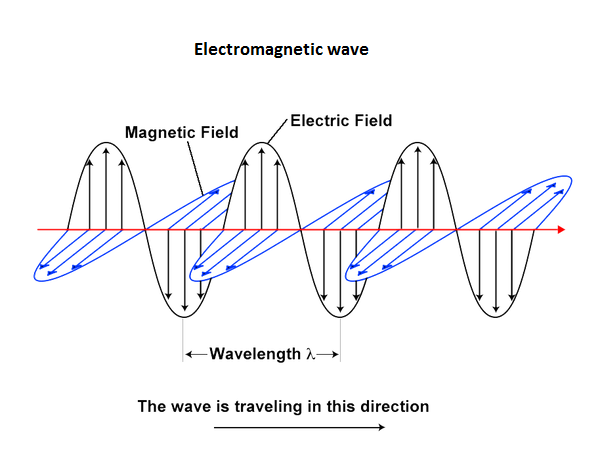
\includegraphics[width=0.75\textwidth]{2-em-wave}
	\caption{Propagation of \gls{em} wave}
	\label{fig:2_em_wave}
\end{figure}
		\subsection{Optical waveguides}
The waveguide is the essential element of every photonic circuit which can be characterized by the number of dimensions in which light is confined inside it \cite{reed_silicon_2008}. A planar waveguide confines light in 1-D, which is simple for understanding of the wave propagation using Maxwell's equations. However, for practical applications 2-D confinement is necessary and that is why channel waveguides are used. Structures like photonic crystals even have 3-D confinement properties.   			
		\subsubsection{Planar waveguides}
A simple planar waveguide consists of a high-index medium with height $h$ surrounded by lower-index materials on the top and bottom sides, known as cladding. The \gls{ri} of the film is $n_f$. The \gls{ri} of the substrate in lower cladding is $n_s$ whereas, \gls{ri} of the substrate in upper cladding is $n_c$.
\begin{figure}[H]
	\centering
	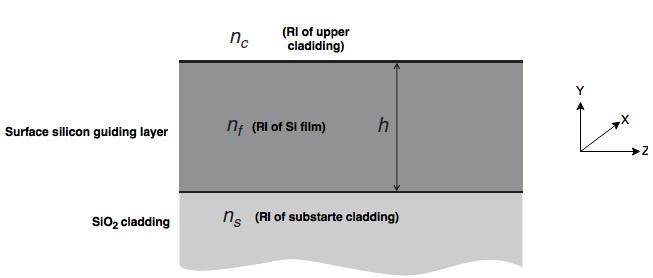
\includegraphics[width=0.75\textwidth]{2-palne-wg}
	\caption{A typical planar waveguide where the film is infinite in XZ-plane}
	\label{fig:2_palne_wg}
\end{figure}
For planar waveguides the wave equation for electric field (\ref{eq:wave_sol_electric}) and magnetic field (\ref{eq:wave_sol_magnetic}) can be rewritten as follows:
\begin{equation}\label{eq:wave_sol_planar_wg}
\begin{aligned}
\begin{cases}
\overrightarrow{E}(z,t)=E_{x}(y)e^{i\left(\omega t \pm k_{0}z\right)}\\
\overrightarrow{H}(z,t)=H_{x}(y)e^{i\left(\omega t \pm k_{0}z\right)}
\end{cases}
\end{aligned}
\end{equation}	
since in X-direction the film is infinite. After using the homogeneous wave equations for a planar waveguide the following \gls{te} and \gls{tm} mode equations can be deduced:
\begin{equation}\label{eq:homogeneous_wave_sol_planar_wg}
\begin{aligned}
\begin{cases}
\nabla^{2}E_x(y) + (k_{0}^{2}n(y)^{2}-k^{2}){E_{x}(y)} = 0\\
\nabla^{2}H_x(y) + (k_{0}^{2}n(y)^{2}-k^{2}){H_{x}(y)} = 0	
\end{cases}
\end{aligned}
\end{equation}
where $n(y)$ depends only on a single Cartesian coordinate $n_{eff} = n(y)$. These equations can be solved analytically using the various boundary conditions of the waveguides which help in deducing the nature of propagation of the wave in \gls{te} and \gls{tm} mode. Different kinds of numerical methods like \gls{fem}, \gls{fit}, \gls{fdtd}, \gls{bpm} have been developed to decipher the nature of light propagation in waveguides.
		\subsubsection{Channel waveguides}			
As mentioned earlier channel waveguides provide confinement in 2-D which helps in analyzing waveguides in a more practical way. The three main types of channel waveguides are rib, strip and buried waveguides. As depicted in \ref{fig:2_rib_wg}, \ref{fig:2_strip_wg}, \ref{fig:2_buried_wg} the different conceptual structures of the waveguides can be envisaged. While the rib and strip waveguides are designed using etching techniques, the buried waveguide mostly relies on diffusion and epitaxial growth techniques for its fabrication.
\begin{figure}[H] %h
	\begin{subfigure}[t]{0.3\textwidth}
		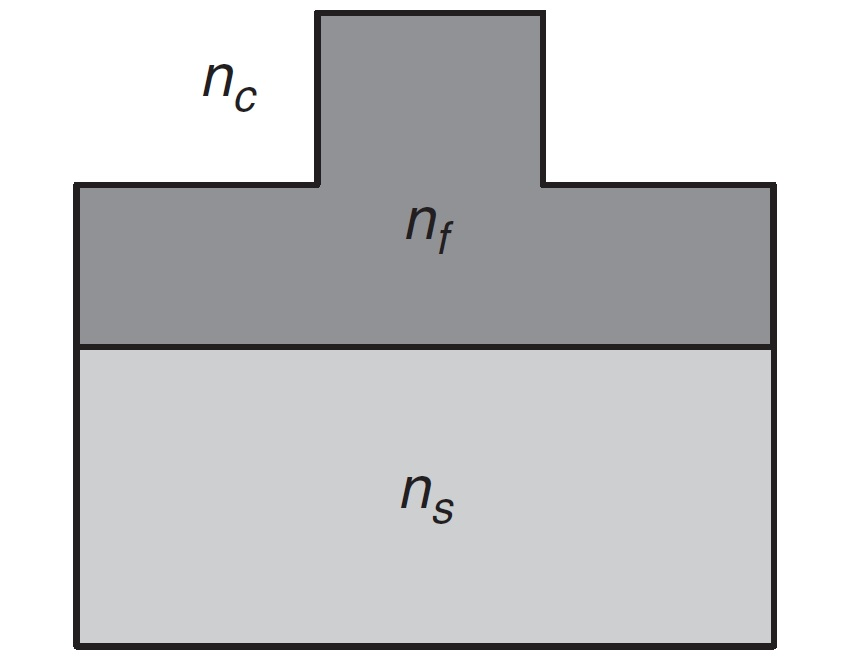
\includegraphics[width=\textwidth]{2-rib-wg}
		\caption{Rib waveguide}
		\label{fig:2_rib_wg}
	\end{subfigure}
	\hfill
	\begin{subfigure}[t]{0.3\textwidth}
		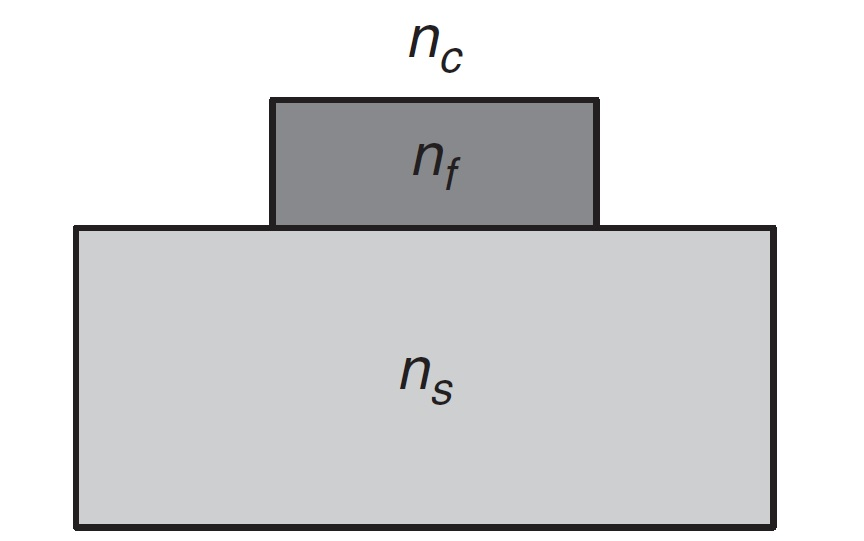
\includegraphics[width=\textwidth]{2-strip-wg}
		\caption{Strip waveguide}
		\label{fig:2_strip_wg}
	\end{subfigure}
	\hfill
	\begin{subfigure}[t]{0.3\textwidth}
		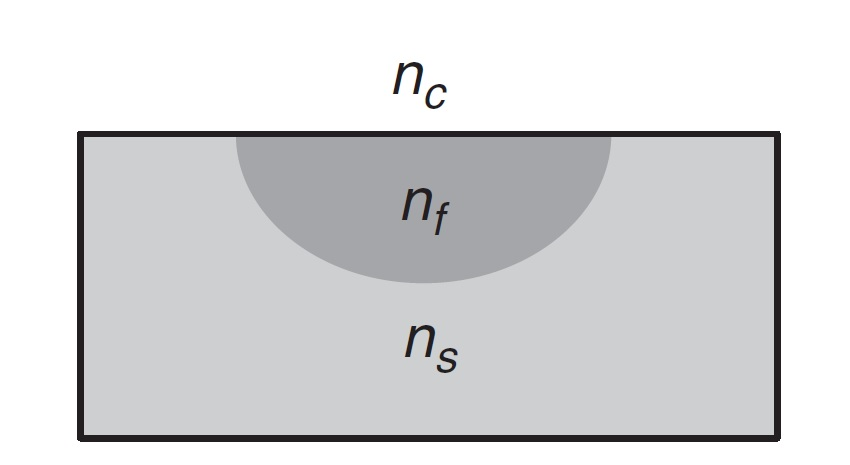
\includegraphics[width=\textwidth]{2-buried-wg}
		\caption{Buried waveguide}
		\label{fig:2_buried_wg}
	\end{subfigure}
	\caption{Different kinds of design for channel waveguides}
\end{figure}
\begin{itemize}	
	\item \textbf{Design rules of rib waveguides:} While designing these waveguides each of these have specific design rules for optimum performance and low-loss coupling, which has been standardized after years of research \cite{reed_silicon_2008}. The \gls{smc} for \textit{rib waveguides} is as follows:	
	\begin{equation}\label{eq:smc_rib_wg}
	\begin{aligned}
	\dfrac {W} {H}\leq 0.3+\dfrac {r} {\sqrt {1-r^{2}}},  && \text{ for } (0.5 \leq r < 1)
	\end{aligned}
	\end{equation}
	where $W$=waveguide width, $H$=rib height, $r$ is ratio of slab height to overall rib height.
	\begin{figure}[H] %h
		\centering
		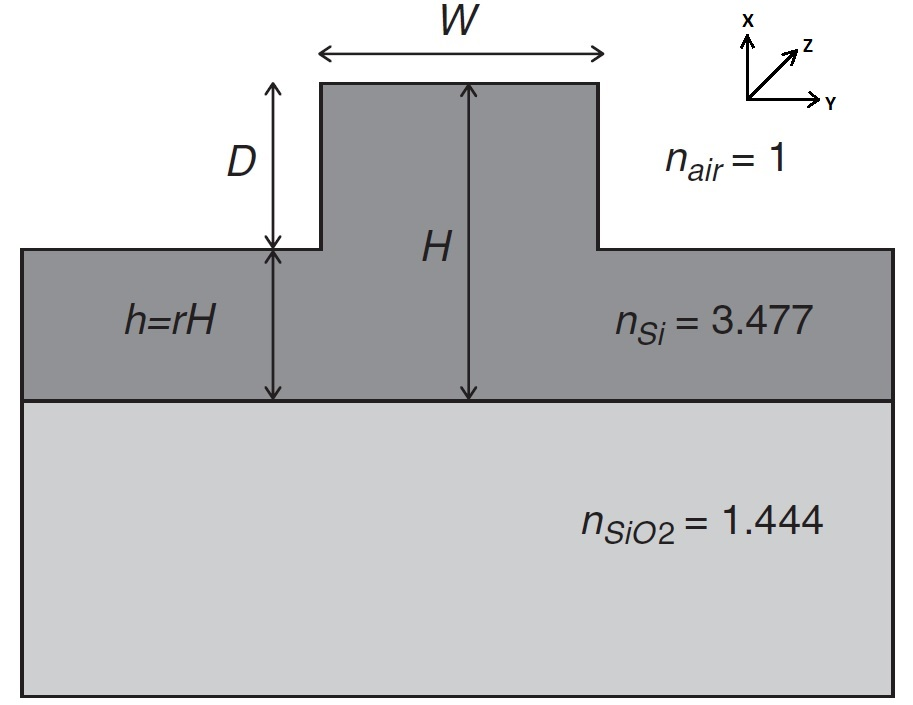
\includegraphics[width=0.75\textwidth]{2-rib-wg-design}
		\caption{Rib waveguide design rules}
		\label{fig:2_rib_wg_design}
	\end{figure}
The main requirements of the waveguide to cater the propagation of waves is that the dimension of the waveguide has to be more than the wavelength of the propagating wave. Depending on the required mode confinement, the width and height are adjusted such that it adheres to \ref{fig:2_rib_wg_design}.
	
\item \textbf{Design rules of strip waveguides:} In mode confinement of light in optical waveguides the effective mode \gls{ri} is important. Strip waveguides offer more high \gls{ri} contrast in comparison to Rib waveguides. This can help in realization of ultra-dense photonic circuits because of high effective mode confinement. This can also achieve small bends which can improve the characterization of different monolithic optical circuits. Sometimes the side walls cannot be etched in a perfectly smooth way causing greater evanescent fields from the waveguides introducing unnecessary coupling and losses. Using simulation for the desired scenario the robust values of the dimensions can be achieved depending on the application.
\end{itemize}
		
		\subsection{Snell's law and total internal reflection}
If light ray propagating in a medium with \gls{ri} $n_1$, impinges on the interface between two media, at an angle $\theta_1$, as shown in Figure \ref{fig:2_snells_law}, the ray is partially transmitted ($E_t$) and partially reflected ($E_r$). The relationship between the \gls{ri}s $n_1$ and $n_2$, and the angles of incidence ($\theta_1$) and refraction ($\theta_2$), is given by Snell's law:
\begin{equation}\label{eq:snells_law}
n_1 \sin \theta_1 = n_2 \sin \theta_2
\end{equation}
\begin{figure}[H]
	\centering
	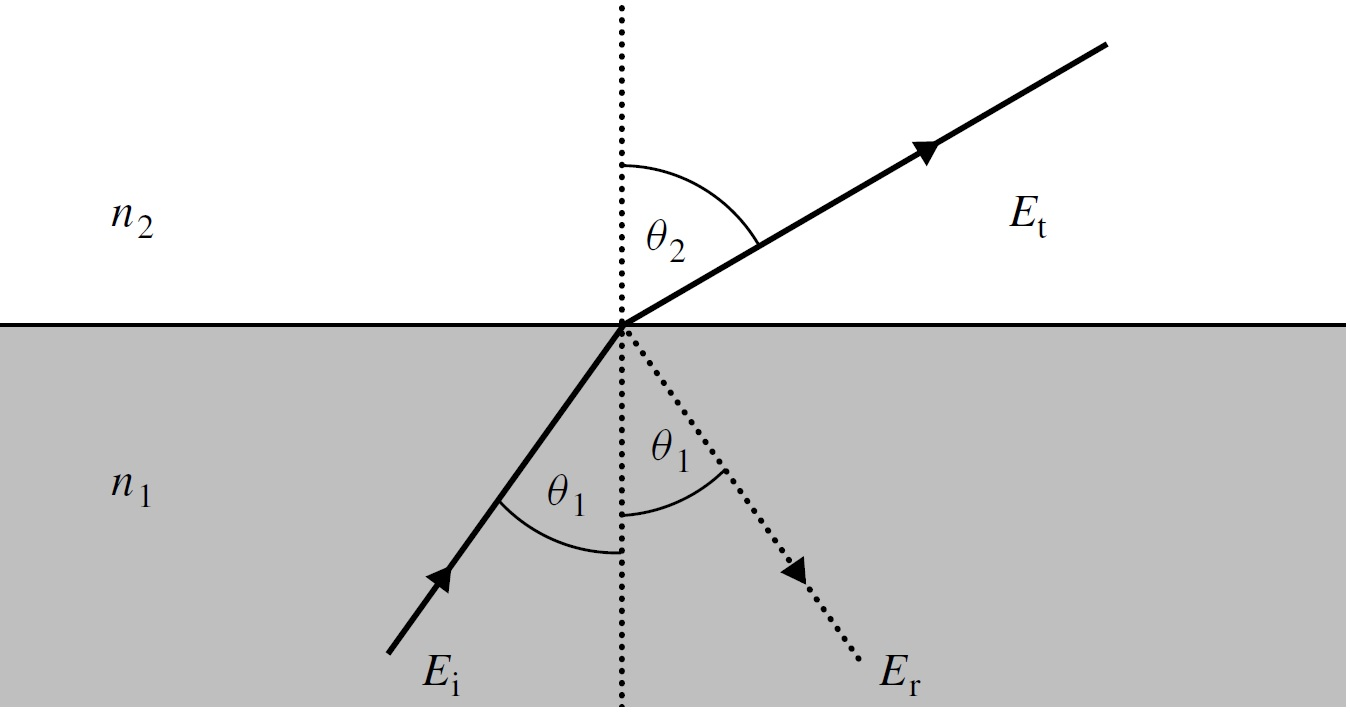
\includegraphics[width=0.75\textwidth]{2-snells-law}
	\caption{Light rays refracted and reflected at the interface of two media}
	\label{fig:2_snells_law}
\end{figure}
For some angle $\theta_1$, the corresponding angle $\theta_2$ will reach $90^{\circ}$, and hence Snell’s law simplifies to:
\begin{equation}\label{eq:critical angle}
\begin{aligned}
\begin{cases}
n_1 \sin \theta_c = n_2\\
\sin \theta_c = \dfrac{n_2}{n_1}
\end{cases}
\end{aligned}
\end{equation}
where, $\theta_c$ is defined as the critical angle. For angles of incidence greater than this critical angle, no light is transmitted and total internal reflection occurs. These properties are important to consider for finding the acceptance angle at which light can be inserted into a waveguide. The ray model helps in understanding of reflection and refraction of light at boundaries between the medium.
		
		\subsection{Eigenvalue and wave modes}
In general, the electric field and magnetic field in the wave equation in \ref{eq:wave_sol_electric} and \ref{eq:wave_sol_magnetic} can be written in its constituent parts in Cartesian coordinates as:
\begin{equation}\label{eq:em_field_cart_cord}
\begin{aligned}
\begin{cases}
\overrightarrow{E}=E_{x}\widehat{x}+E_{y}\widehat{y}+E_{z}\widehat{z}\\
\overrightarrow{H}=H_{x}\widehat{x}+H_{y}\widehat{y}+H_{z}\widehat{z}
\end{cases}
\end{aligned}
\end{equation}
The generalized vectorial component of the electric and magnetic field of equation \ref{eq:homogeneous_wave_sol_planar_wg} for a traveling wave in $Z$ direction can be combined into the Helmholtz equation as follows:
\begin{equation}\label{eq:helmholtz_eq_rib_wg}
	\begin{aligned}
		\nabla ^{2}\Psi \left( x,y,z\right) +k_{0}^{2}n^{2}\left(x,y\right) \Psi \left( x,y,z\right) = 0
	\end{aligned}
\end{equation}
where, $\Psi \left( x,y,z\right) = \psi \left( x,y\right)e^{-jkz} $ and then the equation \ref{eq:helmholtz_eq_rib_wg} can be rewritten as,
\begin{equation}\label{eq:helmholtz_eq_wg_general}
\begin{aligned}
\nabla_{xy} ^{2}\psi \left( x,y\right) +\left(k_{0}^{2}n^{2}\left(x,y\right) - k^2\right)\psi \left( x,y\right) = 0.
\end{aligned}
\end{equation}

\noindent The equation \ref{eq:helmholtz_eq_wg_general} can be solved for $\psi \left( x,y\right)$, using different numerical analysis methods like \gls{fem}, \gls{fit}, \gls{bpm}, \gls{fdtd}. For optical applications, the main used methods are \gls{fem} (Frequency domain solver), \gls{fit} (Time domain solver). The numerical methods first decompose the waveguide into sufficient number small cells (more cells give more robust solution at the cost of increased computing) and then discretization of the refractive index profile is performed. Next the field equations are discretized by replacing the derivatives by their finite difference representations in those cells. In this way a set of linear equations are obtained which can be solved using standard algebraic methods. In general, \gls{fit} has a much lower memory footprint.\par

For given $\omega$, the resulting mode problem is an eigenproblem, solved for eigenvectors, i.e., mode profiles $\psi(x, y)$, and eigenvalues, from which the corresponding propagation constants $k$ of the modes are computed. The geometry of the waveguide is given by the transverse dependence of $\epsilon$, with effective \gls{ri} profile, and by appropriately chosen boundary conditions. Each allowed solution is referred to as the \textit{mode of propagation}. For example, when light travels through a rectangular waveguide different modes can be visualized as follows in Fig. \ref{fig:2_rect_te_modes}.
\begin{figure}[H]
	\centering
	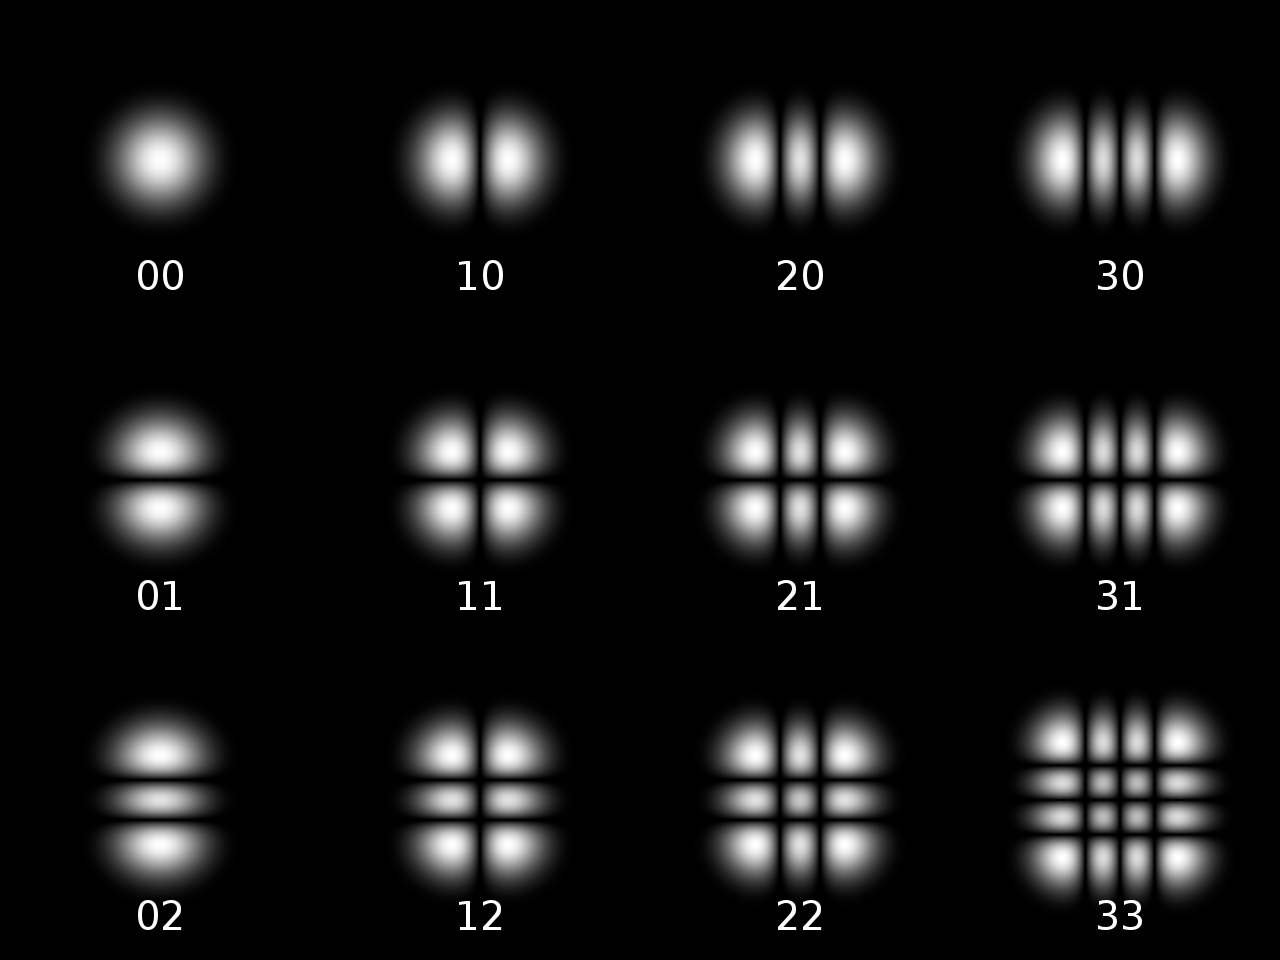
\includegraphics[width=0.75\textwidth]{2-rect-te-modes}
	\caption{Rectangular transverse mode patterns \gls{te}(mn)}
	\label{fig:2_rect_te_modes}
\end{figure}
		
		\subsection{Optical polarization and transverse modes}
In optical waveguides, the transmission distance is limited by several types of dispersion, or spreading of optical pulses as they travel along the waveguide. Dispersion in waveguide is caused by a variety of factors. Intermodal dispersion, caused by the different axial speeds of different transverse modes, limits the performance of multi-mode waveguide. Because single-mode waveguide supports only one transverse mode, intermodal dispersion is eliminated. In single-mode performance is primarily limited by chromatic dispersion (also called group velocity dispersion), which occurs because the \gls{ri} of silicon varies slightly depending on the wavelength of the light. \gls{pmd}, another source of limitation, occurs because although the single-mode waveguide can sustain only one transverse mode, it can carry this mode with two different polarizations, which travel at different propagation velocities. This phenomenon is called birefringence and its effect can be counteracted by polarization-rotator. \gls{pmd} limits the bandwidth of the waveguide because the spreading optical pulse limits the rate that pulses can follow one another on the waveguide and still be distinguishable at the receiver.\par

Polarization is the direction of the electric field associated with the propagating wave. In the example in Fig. \ref{fig:2_em_wave} the wave is linearly polarized since the electric field and magnetic field exist in one direction only. In a dielectric optical waveguide, light propagates in linearly polarized modes and the plane in which light is polarized is either vertical or horizontal to the direction of wave, as shown in Fig. \ref{fig:2_te_tm_mode} in single-mode.
		
			\subsubsection{TE mode}
\gls{te} mode is the fundamental mode in which there is no electric field in the direction of propagation of light wave. In Fig. \ref{fig:2_te_tm_mode} the electric field lines (blue) are perpendicular to the plane of incidence in \gls{te} mode. The plane of incidence is the plane in which optical waves strike the surface of the waveguide.						
			\subsubsection{TM mode}
\gls{tm} mode is the fundamental mode in which there is no magnetic field in the direction of propagation of light. In Fig. \ref{fig:2_te_tm_mode} it can be seen that magnetic field (red lines) are perpendicular to the plane of incidence in \gls{tm} mode.
 
			\subsubsection{Quasi-TE and Quasi-TM mode}				
Practically, waveguide cores have electric and magnetic fields that slice through air and the cladding substrate. Hence they do not support pure \gls{te} and \gls{tm} modes. However, since most the power is contained under the waveguide core and inside just the cladding, \gls{te} and \gls{tm} modes can be a good approximation. Generally, in these modes there is some field component in the direction of propagation as well. This is known as quasi-\gls{te} and quasi-\gls{tm} mode.

\begin{figure}[H]
	\centering
	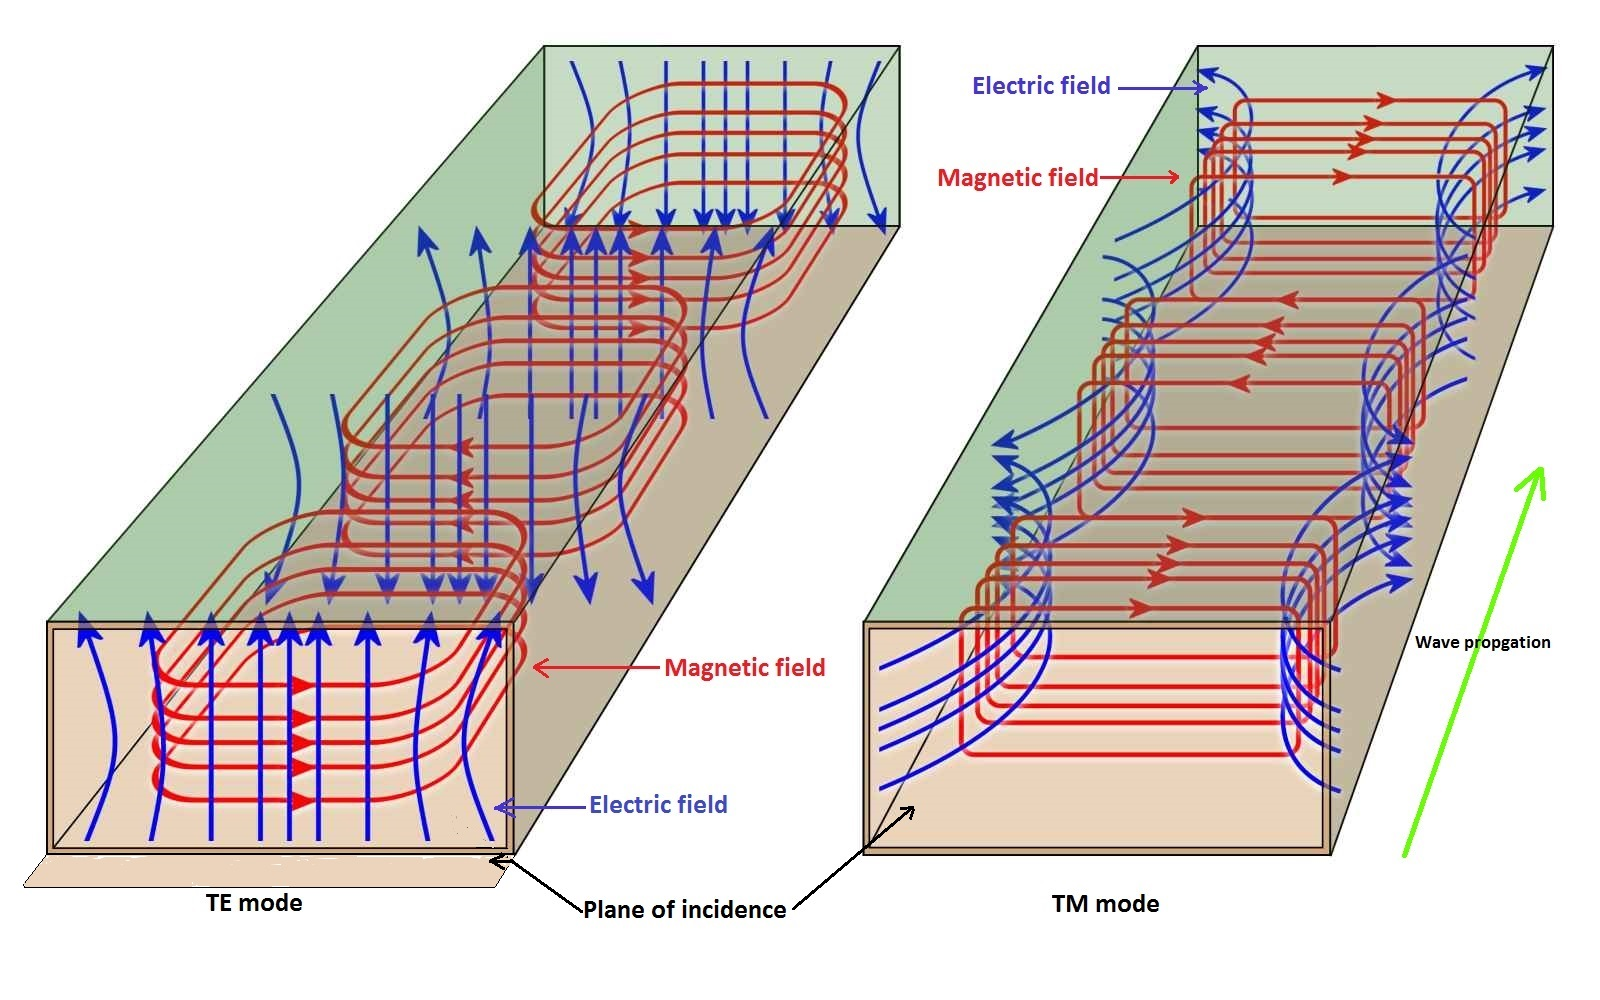
\includegraphics[width=\textwidth]{2-te-tm-mode}
	\caption{\gls{te} and \gls{tm} fundamental mode in a waveguide using CST simulation}
	\label{fig:2_te_tm_mode}
\end{figure}
			
		\subsection{Confinement factor}
Often it is necessary to know the confined power inside the core of the waveguide which helps in figuring out the waveguide mode. The confinement is also a measure of the proportion of the power in a given mode that lies within the core \cite{reed_silicon_2008}.  
\begin{equation}\label{eq:per}
\text{ Confinement factor } = \dfrac {\int _{-H / 2}^{H/2}E_{x}^{2}\left( y\right) dy} {\int _{-\infty }^{\infty }E_{x}^{2}\left( y\right) dy}
\end{equation}
Confinement factor is an important measure which is function of various factors like polarization, \gls{ri} difference between the core and cladding, mode number etc.	
		
		\subsection{Jones calculus}
Polarized light can be represented using Jones calculus. Polarized light is represented using \textit{Jones vector} and linear optical elements are represented by \textit{Jones matrices}.	When light crosses an optical element the resulting polarization of the emerging light is found by taking the product of the Jones matrix of the optical element and the Jones vector of the incident light. \textit{Jones calculus} is only applicable to light that is already fully polarized \cite{burch_introduction_1975}.
		
			\subsubsection{Jones vector}
The Jones vector describes the \gls{sop} of light in free space or another homogeneous isotropic non-attenuating medium, where the light can be properly described as transverse waves \cite{burch_introduction_1975}. The Jones vector is a complex vector that is a mathematical representation of a real wave. A typical representation of the electric field for the optical wave described in \ref{eq:wave_sol_electric} can be as follows:
\begin{equation}\label{eq:jones_vector}
E = \left( \begin{matrix} E_{x}\left( t\right) \\ E_{y}\left( t\right) \\ 0\end{matrix} \right) = \left( \begin{matrix} E_{x}e^{i\left( \omega t - kz+\phi _{x}\right)} \\ E_{y}e^{i\left( \omega t - kz+\phi _{y}\right) }\\ 0\end{matrix} \right) = \left( \begin{matrix} E_{x}e^{i\phi_x}\\ E_{y}e^{i\phi_y}\\ 0 \end{matrix} \right)e^{i\left( \omega t - kz\right)} 
\end{equation}
where $\phi_x$ and $\phi_y$ indicate the phasor notation. The Jones vector of the plane wave is described by:
\begin{equation}\label{eq:jones_vector_form}
\left( \begin{matrix} E_{x}e^{i\phi_x}\\ E_{y}e^{i\phi_y}\end{matrix} \right) 
\end{equation}
and the intensity of the optical, $I$ wave can be written as,
\begin{equation}\label{eq:jones_vector_intensity}
I = \left| E_x\right| ^{2}+\left| E_y\right| ^{2} 
\end{equation}
Generally, when considering Jones vector a wave of unit intensity is required for the consideration polarization, so Jones vector is noted using an unit vector where,
\begin{equation}\label{eq:jones_unit_vector_form}
	E\overline {E} = 1
\end{equation}
where $\overline {E}$ is the complex conjugate of $E$. 
In general the Jones representation of a normalized elliptically polarized beam with azimuth $\theta$ and elliptical angle $\epsilon$ is given by,
\begin{equation}\label{eq:jones_vector_general_form}
e^{i\phi}\left(\begin{matrix} 
\cos\theta\cos\epsilon - j\sin\theta\sin\epsilon\\
\sin\theta\cos\epsilon - j\cos\theta\sin\epsilon 
\end{matrix} \right) 
\end{equation}
where $e^{i\phi}$ is an arbitrary phase vector and $\phi = \phi_x - \phi_y$. So, for example a linear polarization of \gls{te} mode can be represented as,
\begin{equation}\label{eq:jones_vector_linear_pol}
\left(\begin{matrix}  
1 \\
0
\end{matrix} \right) 
\end{equation}
since, $\theta=0$ and $\epsilon = 0$.
			
			\subsubsection{Jones matrix}
Jones matrix is the formal representation of the various optical elements such as lenses, beam splitters, mirrors, phase retarders, polarizers at arbitrary angles that can modify polarization. They generally operate on Jones vector and helps in comprehend situations which light encounters multiple polarization elements in sequence. In these situations the products of the Jones matrices can be used to represent the transfer matrix. This situation can be represented using,
\begin{equation}\label{eq:jones_matrix}
[E_{output}] = J_{system}[E_{input}] 
\end{equation}
where $E_{input}$ is the input field into the optical system and $E_{output}$ is the generated output field represented using Jones vector. The matrix $J_{system}$ is the Jones matrix of the optical system comprising of a series of polarization devices. If there are $N$ devices in the system then the final transfer matrix comes out as,
\begin{equation}\label{eq:jones_transfer_matrix}
J_{system} =J_{N}J_{N-1}\ldots \ldots J_{2}J_{1} 
\end{equation}   
where $J_{N}$ is the Jones matrix for $n^{th}$ polarizing optical element.

			\subsubsection{Jones matrix for polarizing optical systems}
To construct optical waveguides for polarization rotation it is imperative to deal with the basic principles of standard available optical systems. Here, the fundamental principles of polarizer and wave plates are interpreted using Jones calculus.
		\subsubsection*{Polarizer}
Polarizers have an index of refraction which depends on orientation electric field propagation. If any optical system has a transmission axis and an absorption axis for electric fields, then lights will be passed along he transmission axis and absorbed along the other axis. So, the Jones matrix of a polarizer making an angle $\theta$ with the X-axis will come out as,
\begin{equation}\label{eq:jones_matrix_polarizer}
\left(\begin{matrix} 
\cos ^{2}\theta & \sin \theta \cos \theta \\ 
\sin \theta \cos \theta & \sin ^{2}\theta
\end{matrix} \right) 
\end{equation} 
		\subsubsection*{Wave plates}
Wave plates are phase retarders which are made of birefringent crystals. Wave plates can be conceptualized as two polarizers kept apart at certain distance $d$, such that their polarization axes are apart orthogonally ($90^{0}$). The phase difference as light passes through this setup of thickness $d$ is \cite{peatross_physics_2015},
\begin{equation}\label{eq:jones_matrix_wp1}
\left(k_{slow}-k_{fast}\right)d = \dfrac {2\pi d} {\lambda_{vac} }\left( n_{slow}-n_{fast}\right) 
\end{equation}
In, general the Jones matrix for a wave plate is given by \cite{peatross_physics_2015},
\begin{equation}\label{eq:jones_matrix_wp2}
\left( \begin{matrix} 
\cos ^{2}\theta +\xi \sin ^{2}\theta & \sin \theta \cos \theta -\xi \sin \theta \cos \theta\\ 
\sin \theta \cos \theta -\xi \sin \theta \cos \theta & \sin ^{2}\theta +\xi \cos ^{2}\theta
\end{matrix} \right) 
\end{equation}
where $\xi$ is calculated based on the type of wave plate. The following equations addresses some general scenarios:
\begin{equation}\label{eq:jones_matrix_wp3}
\begin{aligned}
\begin{cases} 
\xi = e^{i\pi/2}, \,\quad \text{where,} \left(k_{slow}-k_{fast}\right)d = \pi/2 + 2\pi m, \text{for quarter-wave plate}\\ 
\xi = e^{i\pi},  \;\;\;\quad \text{where,} \left(k_{slow}-k_{fast}\right)d = \pi + 2\pi m, \text{for half-wave plate}
\end{cases}
\end{aligned}
\end{equation}
and $m \in \mathbb{Z}$. $\xi$ is the phase delay of the wave plates. Similar concept is used in the construction of \gls{pr} waveguides which will be discussed in later sections shortly.
 		
		\subsection{Poincaré sphere and state of polarization} \label{concept:poincare_sphare}
To view a complete representation of all the polarization ellipses generated using Jones vectors, a spherical structure with unit radius is used, which is known as Poincaré sphere. If the orientation in space of of the ellipse of polarization is determined by the azimuth, $\theta$ and ellipticity, $\epsilon$ then that point can be completely characterized by its longitude $2\theta$ and latitude $2\epsilon$. The north and south poles represent the right-handed and left-handed circular polarization respectively. In general the diametrically opposite points represent pairs of orthogonal polarization. The \gls{sop} and its corresponding location in the Poincaré sphere is visualized in the Fig. \ref{fig:2_poincare}. To go from one \gls{sop} to another the polarized light can be passed through various optical components which can be computed using the Jones matrix and the corresponding \gls{sop} can be depicted on the Poincaré sphere as well. 
\par The \gls{sop} of any wave are \gls{fom} for \gls{pr} and are described using \textbf{\gls{per}} and polarization phase, $\phi$ given by the following equations:
\begin{equation}\label{eq:wave_sop}
\begin{aligned}
\begin{cases}
PER_{TE-TM} = 10\log \dfrac {P_{TM}} {P_{TE}}\\
PER_{TM-TE} = 10\log \dfrac {P_{TE}} {P_{TM}}\\
\phi =\phi _{x}-\phi _{y}
\end{cases}
\end{aligned}
\end{equation}
     
\begin{figure}[H]
	\centering
	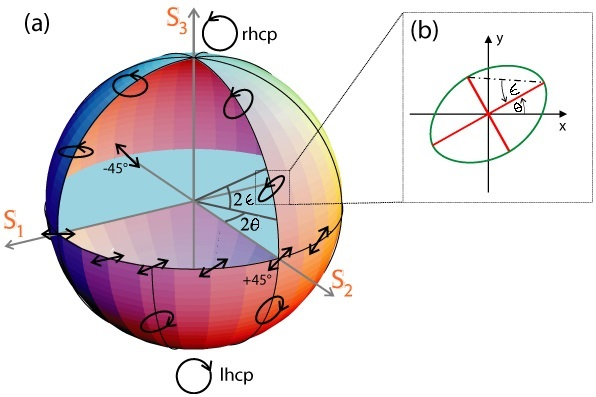
\includegraphics[width=0.75\textwidth]{2-poincare}
	\caption{(a) Representation of the Poincaré sphere (b) Representation of the ellipse parameters \cite{flossmann_stokes_2006}}
	\label{fig:2_poincare}
\end{figure}
\noindent For complete polarized light, the point on the Poincaré sphere must be fixed on time which requires,
\begin{equation}\label{eq:polarization_condition_1}
\dfrac {E_{x}\left( t\right) } {E_{y}\left( t\right) }=constant
\end{equation}
and,
\begin{equation}\label{eq:polarization_condition_2}
\phi = \phi_{x}(t) - \phi_{y}(t)=constant
\end{equation}
\par Apart from the afore mentioned \gls{fom}, another important characteristic which must be optimized is \textbf{Insertion loss}. It is the loss of signal power resulting from the insertion of a device in a transmission line or optical fiber and is usually expressed in decibels (dB). If the power transmitted to the load before insertion is $P_T$ and the power received by the load after insertion is $P_R$, then the \gls{il} in dB is given by,
\begin{equation}\label{eq:insertion_loss}
\gls{il} (dB) = 10\log _{10} \dfrac {P_{T}} {P_{R}}
\end{equation}
  
		\subsection{Stoke's parameter} 		
Quasi-monochromatic waves are mathematically treated using Stokes parameters ($S_0,S_1,S_2,S_3$), which constitute a vector generally known as Stokes vectors. Stokes vectors are used to keep track of the partial polarization (and attenuation) of a light beam in terms of total intensity (I), degree of polarization (p) and ellipse parameters, as the light progresses through an optical system. A Stokes vector can generally be represented as,
\begin{equation}\label{eq:stokes_vector}
\overrightarrow {S} = \left(\begin{matrix}  
	S_0 \\
	S_1 \\
	S_2 \\
	S_3
\end{matrix} \right) 
\end{equation}
where,
\begin{equation}\label{eq:stokes_parameters}
\begin{aligned}
\begin{cases}
S_{0}=I\\ 
S_{1}=I_{p}\cos 2\theta \cos 2\epsilon \\
S_{2}=I_{p}\sin 2\theta \cos 2\epsilon \\
S_{3}=I_{p}\sin 2\epsilon
\end{cases}
\end{aligned}
\end{equation}
Here, $I_p, 2\theta, 2\epsilon$ are the spherical coordinates of the 3-D vector of Cartesian coordinates $(S_1,S_2,S_3)$. So, given the Stokes parameters, the spherical coordinates $(p,2\theta,2\epsilon)$ can be obtained and represented by a point inside the Poincaré sphere using the following:
\begin{equation}\label{eq:stokes_spherical_coordinates}
\begin{aligned}
\begin{cases}
I = S_{0}\\ 
p = \dfrac {\sqrt {S_{1}^{2}+S_{2}^{2}+S_{3}^{2}}} {S_{0}} \\
2\theta = \tan^{-1}\dfrac {S_{2}} {S_{1}} \\
2\epsilon = \tan ^{-1}\dfrac {S_{3}} {\sqrt {S_{1}^{2}+S_{2}^{2}}}
\end{cases}
\end{aligned}
\end{equation}
The prescribed notations are portrayed on the Poincaré sphere in the following Fig. \ref{fig:2_stoke_param_poincare_sphere}.    
\begin{figure}[H]
	\centering
	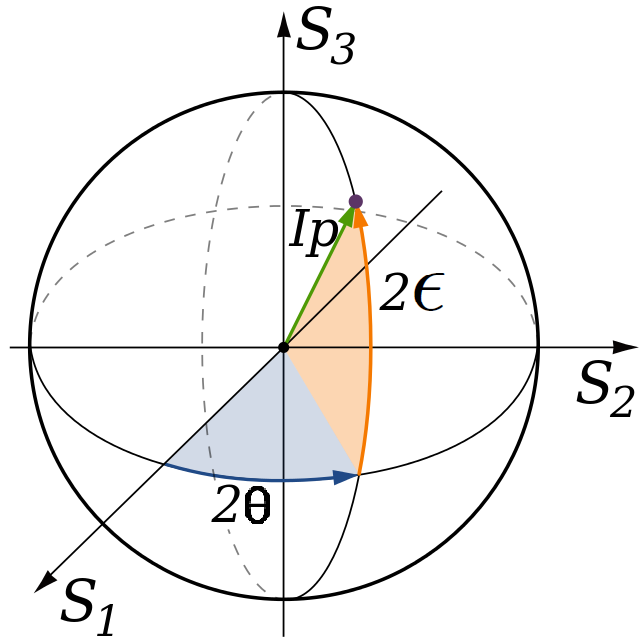
\includegraphics[width=0.50\textwidth]{2-stoke-param-poincare-sphere}
	\caption{Poincaré sphere, on or beneath which the three Stokes parameters [S1, S2, S3] are plotted in Cartesian coordinates \cite{stoke_poincare_parameter}}
	\label{fig:2_stoke_param_poincare_sphere}
\end{figure}

	\subsection{Coupling mode theory}\label{concept:mode_coupling}
In a waveguide, an ideal mode is an eigenvector of a propagation constant. Mode coupling enables transfer of energy from one ideal mode to another, during propagation. Mode coupling can be induced by introducing randomness in the waveguide. This can be achieved through random or intentional index perturbations, bends and stresses within a waveguide, or by introducing another independent waveguide structure in close proximity (coupled waveguides in close proximity are modeled as a single structure, forming supermodes). The pairwise coupling strength between two modes depends on a dimensionless ratio between the coupling coefficient (per unit length) and the difference between the two modal propagation constants. Hence, a given perturbation may strongly couple modes having nearly equal propagation constants, but weakly couple modes having highly unequal propagation constants. \gls{pmd} and \gls{pdl} have long been described by field coupling models, in which phase dependent coupling of modal fields is described by complex coefficients. Field coupling models describe not only a redistribution of energy among modes, but also how eigenvectors and their eigenvalues depend on the mode coupling coefficients \cite{kahn_mode_2012}.

\paragraph*{Perturbation Analysis:}
Supermodes can be represented as weighted sum of individual guided modes. If two modes are represented by $\psi_1(x,y)$ and $\psi_2(x,y)$ in the different waveguides along with the coupling between two modes as $X_i(z)$, then the supermode can be written using Helmholtz identity as, 
\begin{equation}\label{eq:supermodes}
	\Psi(x,y,z) = X_1(z)\psi_1(x,y) + X_2(z)\psi_2(x,y)
\end{equation} 	
The uncoupled modes, $\psi_1$ and $\psi_2$ satisfy the following propagation equations with propagation constants $k_1$ and $k_2$,
\begin{equation}\label{eq:uncoupled_mode}
\begin{aligned}
\begin{cases}
\dfrac {dX_{1}} {dz}=-jk_{1}X_{1} \\[10pt]
\dfrac {dX_{2}} {dz}=-jk_{2}X_{2}
\end{cases}
\end{aligned}
\end{equation}
A known solution for \ref{eq:uncoupled_mode} is:
\begin{equation}\label{eq:uncoupled_mode_sol}
\begin{aligned}
\begin{cases}
X_{1} (z) = e ^ {-jk_{1}z} \\
X_{2} (z) = e ^ {-jk_{2}z}
\end{cases}
\end{aligned}
\end{equation}
Coupled mode theory postulates that to describe a perturbed system the linear coupling terms need to be added as,
\begin{equation}\label{eq:coupled_mode_sol}
\begin{aligned}
\begin{cases}
\dfrac {dX_{1}} {dz} = -jk_{1}X_{1}(z) - j(\kappa_{11}X_1+\kappa_{12}X_2) \\[10pt]
\dfrac {dX_{2}} {dz} = -jk_{2}X_{2}(z) - j(\kappa_{21}X_1+\kappa_{22}X_2)
\end{cases}
\end{aligned}
\end{equation}
where, $\kappa_{ij}$, $\forall \left( i,j\right) \in \left[ 1,2\right] $  are the linear coefficients which can be understood using the scattering matrix as,
\begin{equation}\label{eq:scattering_matix_coupler}
\left(\begin{matrix} 
\kappa_{11} & \kappa_{12} \\ 
\kappa_{21} & \kappa_{22}
\end{matrix} \right) 
\end{equation} 
where,
\begin{equation}\label{eq:coupled_mode_coupling_coeff}
\begin{aligned}
\begin{cases}
\kappa_{11} = \dfrac{1}{2}k_0^2\int\int(n_{12}^2-n_{1}^2)\psi_1^2dxdy \\[10pt]
\kappa_{12} = \dfrac{1}{2}k_0^2\int\int(n_{12}^2-n_{1}^2)\psi_1\psi_2 dxdy \\[10pt]
\kappa_{21} = \dfrac{1}{2}k_0^2\int\int(n_{12}^2-n_{2}^2)\psi_1\psi_2 dxdy \\[10pt]
\kappa_{22} = \dfrac{1}{2}k_0^2\int\int(n_{12}^2-n_{2}^2)\psi_2^2 dxdy
\end{cases}
\end{aligned}
\end{equation}	
Here, $\kappa_{11}$ and $\kappa_{22}$ are the reflection coefficients and $\kappa_{12}$ and $\kappa_{21}$ are the coupling coefficients. Normally, it is assumed that the modes are normalized, and propagate in a lossless system with symmetric coupling coefficients. Hence,
\begin{equation}\label{eq:symmetric_coupling_coeff}
\kappa_{12} = \kappa_{21} 
\end{equation}
Coupling coefficients and phase mismatch are important factors for power exchange between different modes. In \ref{fig:2_mc_theory_1} both the waveguides are excited where as in \ref{fig:2_mc_theory_2} only waveguide $B$ is excited.\todo{Change this pic with some other diagram or simulations..}
\begin{figure}[H]
	\begin{subfigure}[t]{0.45\textwidth}
		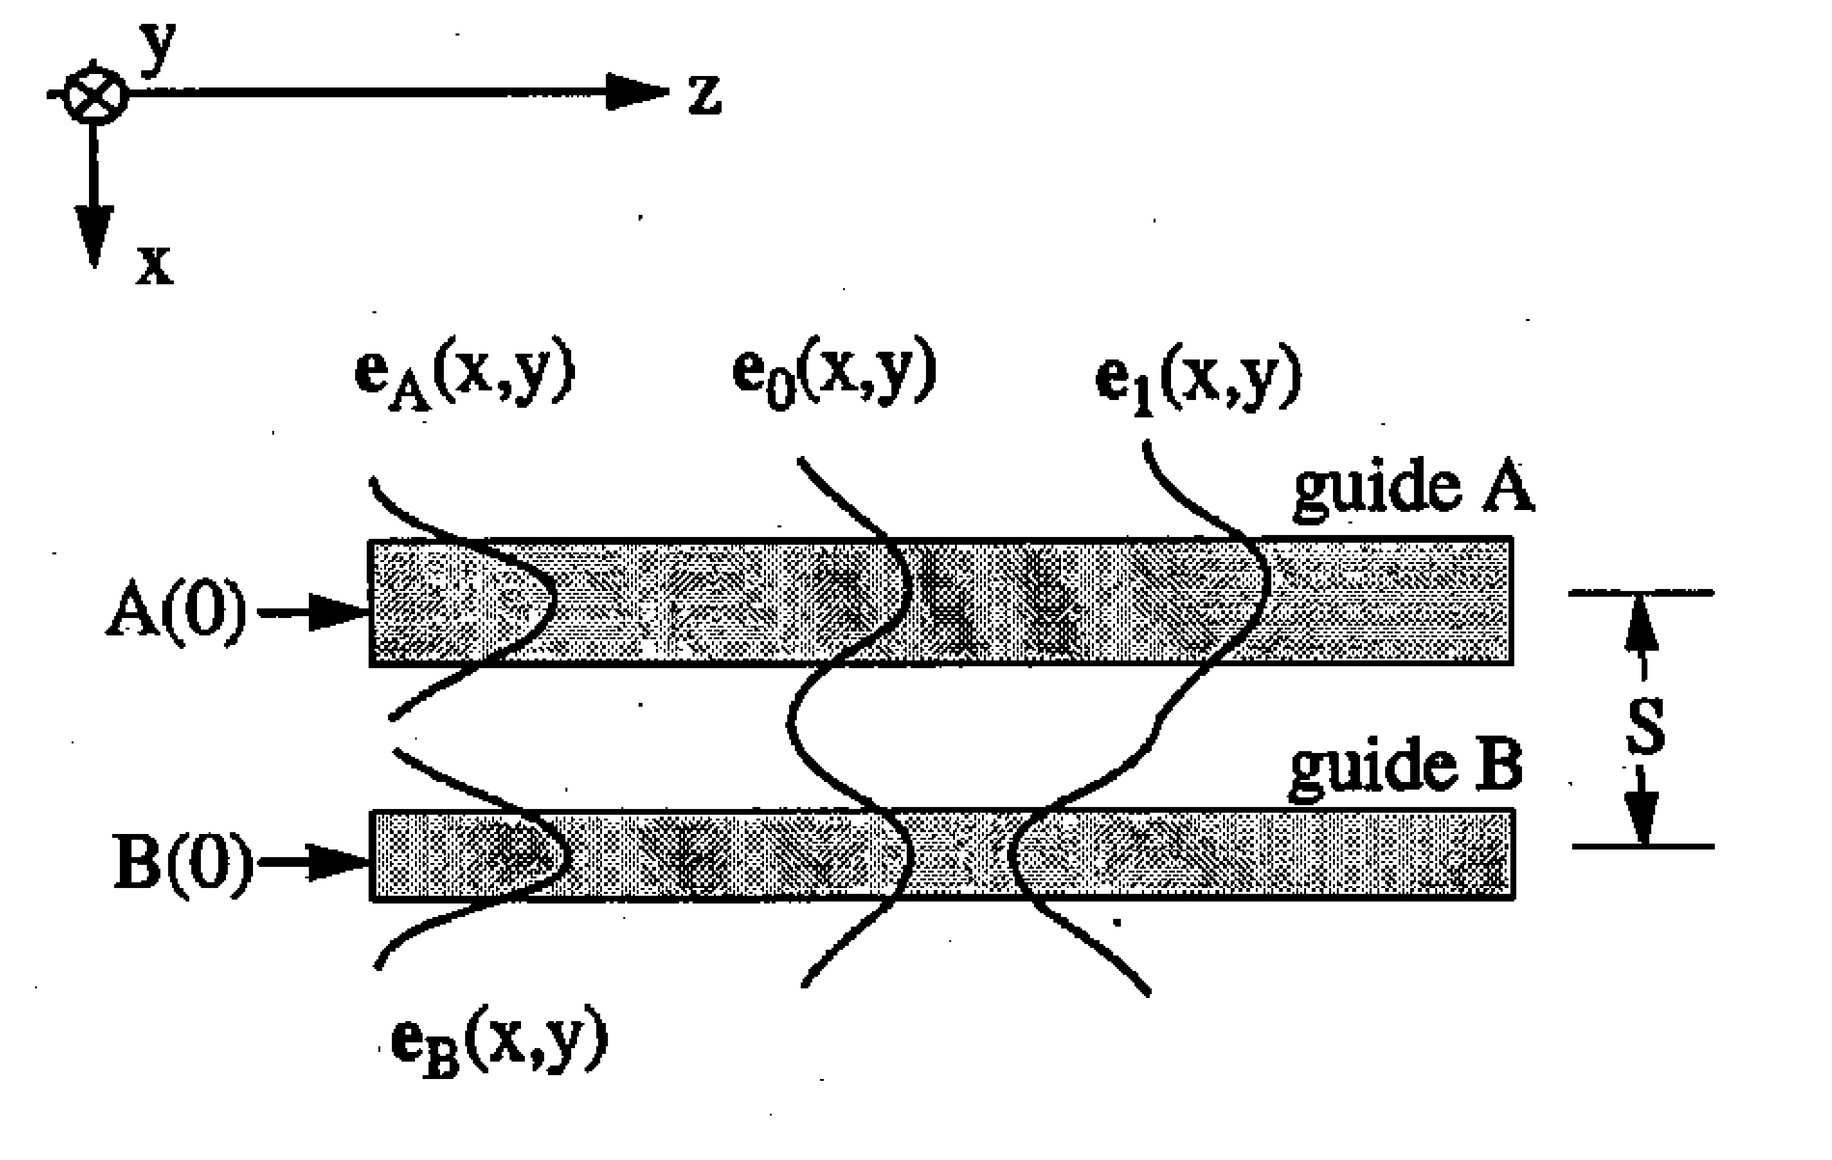
\includegraphics[width=\textwidth]{2-mc-theory-1}
		\caption{Individual and normal modes in two different waveguides}
		\label{fig:2_mc_theory_1}
	\end{subfigure}
	\hfill
	\begin{subfigure}[t]{0.45\textwidth}
		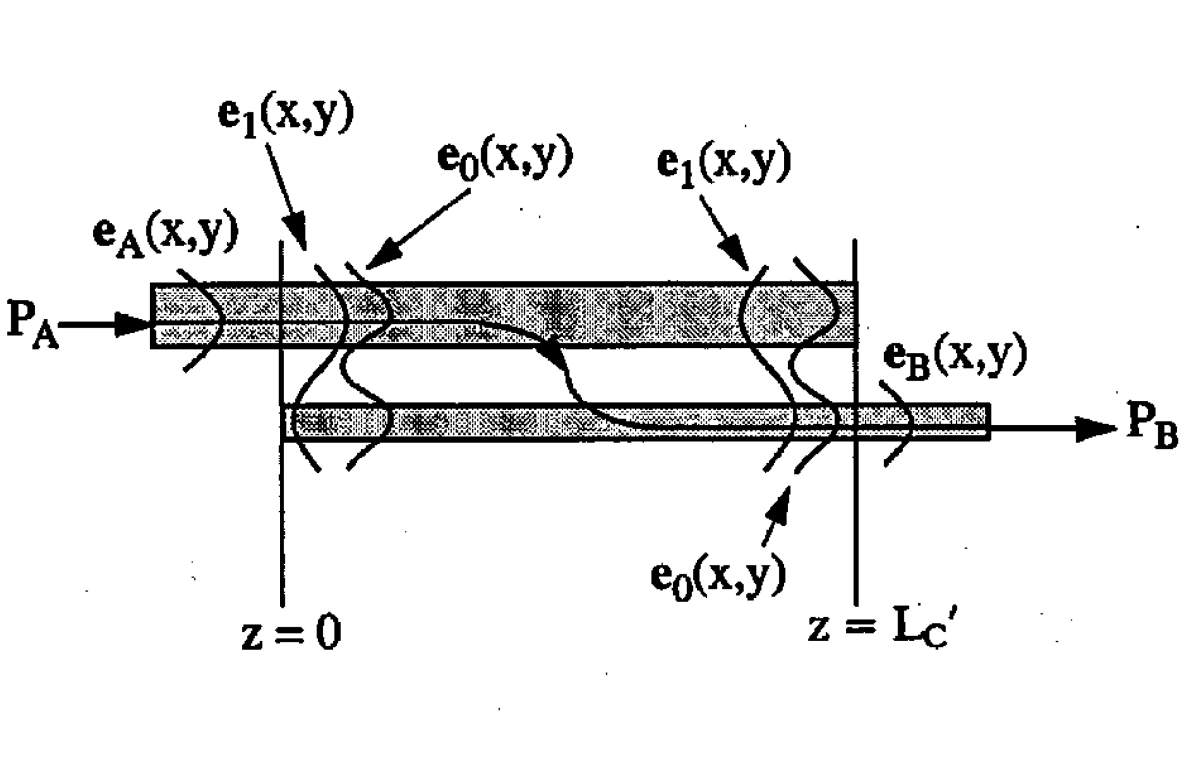
\includegraphics[width=\textwidth]{2-mc-theory-2}
		\caption{Power transfer from arm $A$ to arm $B$ by normal-mode coupling}
		\label{fig:2_mc_theory_2}
	\end{subfigure}
	\caption{Description of the directional coupler under coupled-mode and normal-mode}
\end{figure}

\noindent In \ref{fig:2_mc_theory_2} for no phase mismatch complete power exchange occurs. This is why phase matching is an important criteria for mode coupling. The coupling length, $L_c = \pi / 2\kappa$. 

\par 
Coupling mode theory has been successfully applied to the modeling and analysis of various guided-wave optoelectronic devices, such as optical directional couplers made of thin film and channel waveguides, multiple waveguide lenses, phase-locked laser arrays, distributed feedback lasers and distributed Bragg reflectors, grating waveguides and couplers, nonparallel and tapered waveguide structures, Y-branch waveguides, \gls{te}/\gls{tm} polarization converters, mode conversion and radiation loss in slab waveguides, residual coupling among scalar modes. It has also been used to study the wave coupling phenomena in nonlinear media such as harmonic generation in bulk and guided-wave devices, and nonlinear coherent couplers \cite{haus_coupled_1991}.
	
	\section{Polarization tuning in optical waveguide}
	\todo{Should this section be written in context of polarization tuning? Should it go after PR?}
		\subsection{Thermo-optic mechanism}
		Mach-Zehnder...?? \todo{Is it there?..check}
		
		\subsection{Electro-optic mechanism}
		Mach-Zehnder...? \todo{Is it there?..check}
		
		\subsection{Liquid crystals mechanism}
		
		\subsection{Current injection mechanism}
		
		\subsection{MEMS}
		\todo{Why is MEMS better?}Actuation principle... 	
			
	\section{Polarization rotator (PR)}
For an overall robust network, \gls{pr}s are necessary in optical fiber and \gls{oeic}, which are realized in different approach.	
	\subsection{Optical fiber PR}
	\todo{Write about the PR in optical fiber short with industry standards..}
	Check here..\href{http://www.amstechnologies.com/es/products/optical-technologies/equipment/fiber-optic-test-measurement/measurement-of-fiber-properties/polarisation-mode/view/electrically-driven-polarization-controllers-scramblers/}{Industry standards..}
	\todo{I am not sure how to approach this section}
	
	\subsection{On-chip PR}
The currently available \gls{oeic} \gls{pr}s can be classified under two categories as passive and active \gls{pr}. In the passive \gls{pr}s the waveguide structures are designed in a specific way to manipulate the effective \gls{ri} of the waveguide, in order to obtain the desired polarization. The \gls{ri} cannot be manipulated or tuned once fabricated. Whereas, in active \gls{pr}s, the effective \gls{ri} can be manipulated by thermo-optic or quantum effects.
	
		\subsubsection{Passive PR}
The fields in \gls{te} and \gls{tm} mode are orthogonal (i.e. no coupling exists) and are of different geometry. Thus asymmetric structure in both horizontal and vertical directions are required to break the symmetry, which is accomplished by using different principles viz. mode coupling \cite{dai_novel_2011,ding_Integrated_2013,wang_design_2014}, mode evolution \cite{zhang_selected_2010,chen_compact_2011,zhang_efficient_2012,justin_conference_2012,kazuhiro_integrated_2015} and mode hybridization \cite{fukuda_integrated_2008,leung_numerical_2011,vermeulen_Silicon_2012,velasco_ultracompact_2012}, described in the following sections. All these principles are based on the coupling mode theory described in \ref{concept:mode_coupling}.
			
			\paragraph*{Mode coupling:} Mode coupling \gls{pr} includes a pair of waveguides running parallel to each other, with coupled evanescent fields within close proximity. When two modes with orthogonal polarizations have equal effective \gls{ri}s, strong mode coupling occurs in between the waveguides (generally asymmetric directional couplers), and with proper taper orientation and design, length of coupling region, one mode can be effectively converted to the other.
\begin{itemize}[leftmargin=*]
	\item[$\square$] \begin{minipage}[t]{\textwidth}\textbf{Design: Ultra-compact polarization splitter-rotator based on silicon nanowires}
	\begin{figure}[H] %h
		\begin{subfigure}[t]{0.45\textwidth}
			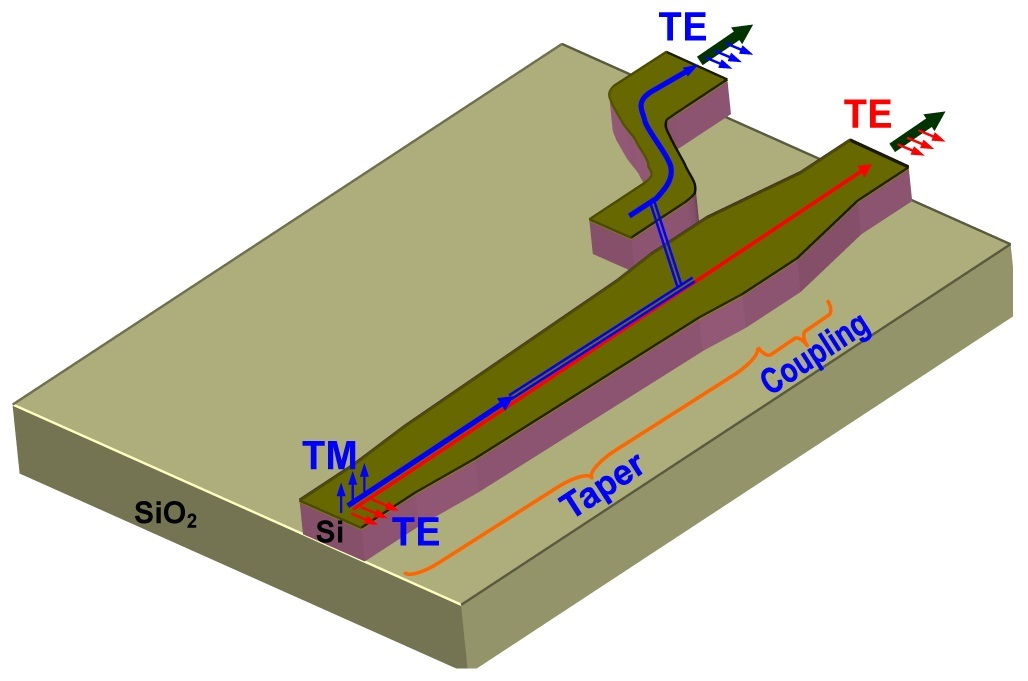
\includegraphics[width=\textwidth]{2-mc-1-1}
			\caption{Schematic of the \gls{pr}}
			\label{fig:2_mc_1_1}
		\end{subfigure}
		\hfill
		\begin{subfigure}[t]{0.45\textwidth}
			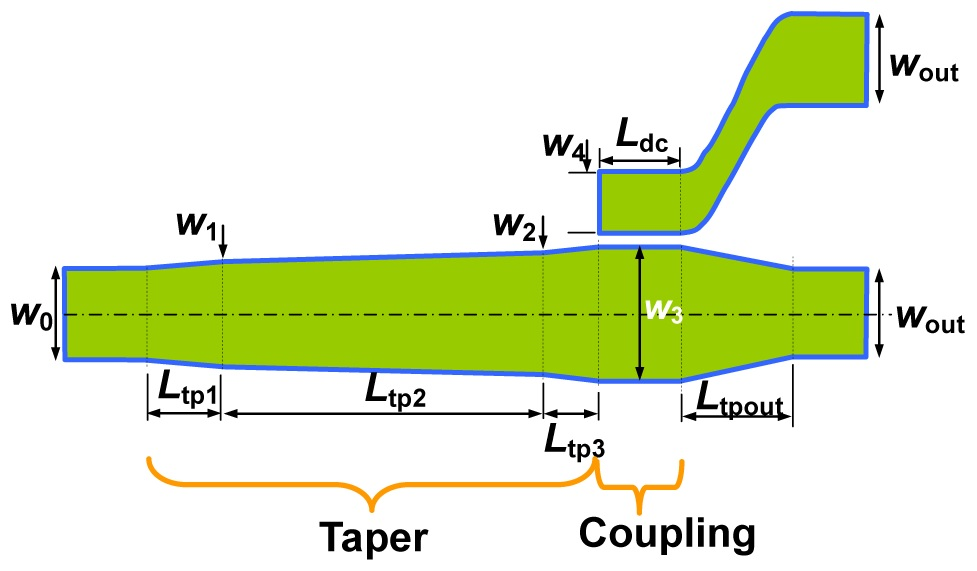
\includegraphics[width=\textwidth]{2-mc-1-2}
			\caption{Structure of the \gls{pr}}
			\label{fig:2_mc_1_2}
		\end{subfigure}
		\caption{\gls{pr} using mode coupling, by Dai and Bowers \cite{dai_novel_2011}}
	\end{figure}
	\end{minipage}\\\\
	\noindent The coupler (Fig. \ref{fig:2_mc_1_1}) consists of 2 waveguides parallel to each other. The section where coupling occurs is shown in Fig. \ref{fig:2_mc_1_2}. The taper structure is singlemode at the input end ($W_0$) while it becomes multimode at the other end ($W_3$). When light propagates along the taper structure, the \gls{tm} fundamental mode launched at the narrow end ($W_0$) is converted to the first higher-order \gls{te} mode at the wide end ($w_3$) because of the mode coupling between them. Another narrow optical waveguide ($W_4$) is then placed close to the wide waveguide ($W_3$) and an asymmetrical directional coupler is formed. By using this asymmetrical directional coupler, the first higher-order \gls{te} mode in the wide waveguide is then coupled to the \gls{te} fundamental mode of the adjacent narrow waveguide. In this way, the input \gls{tm} fundamental mode at the input waveguide is finally converted into the \gls{te} fundamental mode at the cross port of asymmetrical directional coupler. On the other hand, the input \gls{te} polarization keeps the same polarization state when it goes through the adiabatic taper structure. In the region of the asymmetrical directional coupler, the \gls{te} fundamental mode in the wide waveguide could not be coupled to the adjacent narrow waveguide because of the phase mismatching. In this way, \gls{te}- and \gls{tm}- polarized light are separated while the \gls{tm} fundamental mode is also converted into TE fundamental mode \cite{dai_novel_2011}.\par	

	Various other designs for mode coupling have also been proposed \cite{wang_design_2014,ding_Integrated_2013}, which work on the same principle.
	
	\item[$\square$] \textbf{Problem of mode coupling:} The main problem of mode coupling is that directional couplers are not very broadband. Moreover, due to the large birefringence of silicon waveguides, the conversion usually occurs between fundamental \gls{tm} and high order \gls{te} modes and subsequently the high order \gls{te} mode is converted to the fundamental \gls{te} mode.
\end{itemize}		
			\paragraph*{Mode evolution:}
The mode evolution based \gls{pr} includes a single waveguide core. The waveguide is designed in such a way that the cross-section of the waveguide varies along the direction of propagation, both in width and height. This changes polarization from \gls{te} to \gls{tm} or vice versa gradually in propagation direction, under adiabatic transition conditions. Since, the cross-section changes gradually and not abruptly, the \gls{per} is high in these type of \gls{pr}s.

\begin{itemize}[leftmargin=*]
	%\item[$\square$] \begin{minipage}[t]{\textwidth}
	\item[$\square$] \begin{minipage}[t]{\textwidth}\textbf{Design A: Mode evolution \gls{pr} based on single taper}
	\begin{figure}[H] %h
		\begin{subfigure}[t]{0.45\textwidth}
			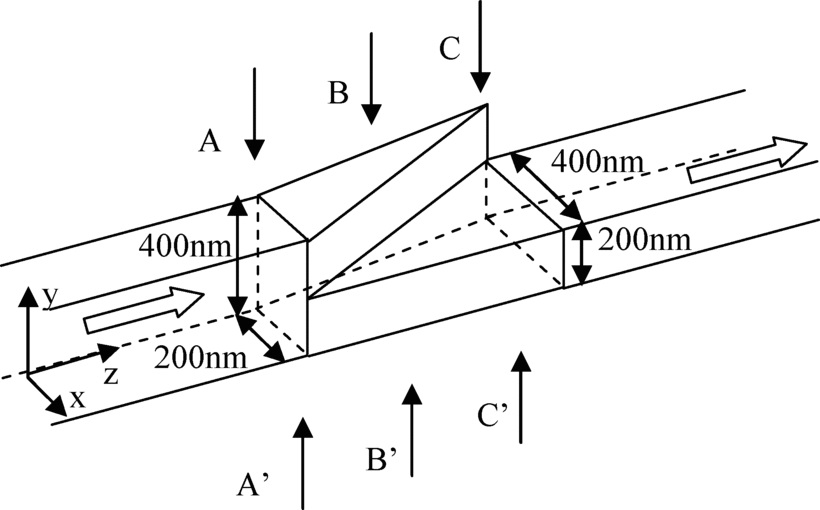
\includegraphics[width=\textwidth]{2-me-2-1}
			\caption{Schematic of the \gls{pr}}
			\label{fig:2_me_2_1}
		\end{subfigure}
		\hfill
		\begin{subfigure}[t]{0.45\textwidth}
			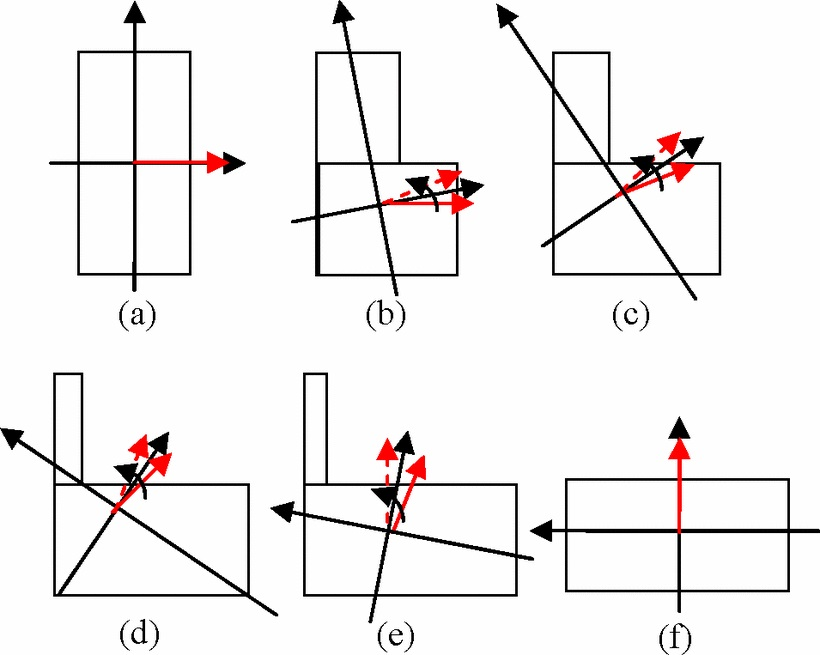
\includegraphics[width=\textwidth]{2-me-2-2}
			\caption{Cross sections of the waveguide at A-A'(a), B-B'(c), and C-C'(f) along with the transition states of the polarization}
			\label{fig:2_me_2_2}
		\end{subfigure}
		\caption{\gls{pr} using mode evolution, by Zhang \textit{et al.} \cite{zhang_selected_2010}}
	\end{figure}
	\end{minipage}\\\\
	\noindent The \gls{pr} (Fig. \ref{fig:2_me_2_1}) consists of the  variable cross section for polarization rotation. The transition region of the rotator was divided into N sections. Each section was considered as a uniform asymmetrical waveguide like the rotator in \cite{wang_ultrasmall_2008}. The length of each section was its half-beat length. The half-beat length of the $n^{th}$ section is $L_{\pi }^{n}=\left( \pi  / \left( \beta _{1}^{n} - \beta _{2}^{n}\right) \right)$ , where $\beta ^{n}=\left( 2\pi / \lambda \right) n_{eff}^{n}$ and $\beta _{1}^{n}$ and $\beta _{2}^{n}$ are the propagation constants of the two fundamental modes in the $n^{th}$ section. After propagating in the $n^{th}$ section, the polarization will rotate $2\Delta \varphi _{n}$ toward the optical axis, where $\varphi _{n}$ is the angle between the optical axis and the polarization of the incident light. The overall rotator should satisfy $\sum _{n}2\Delta \varphi _{n}=90^{0}$, to achieve a rotation of $90^{0}$ in the cascaded sections. Fig. \ref{fig:2_me_2_2} shows the rotation procedure \cite{zhang_selected_2010}.
	%\end{minipage}
			
	\item[$\square$] \begin{minipage}[t]{\textwidth}\textbf{Design B: Mode evolution \gls{pr} composed of an asymmetric-rib waveguide and a tapered waveguide}
	\begin{figure}[H] %h
		\begin{subfigure}[t]{0.45\textwidth}
			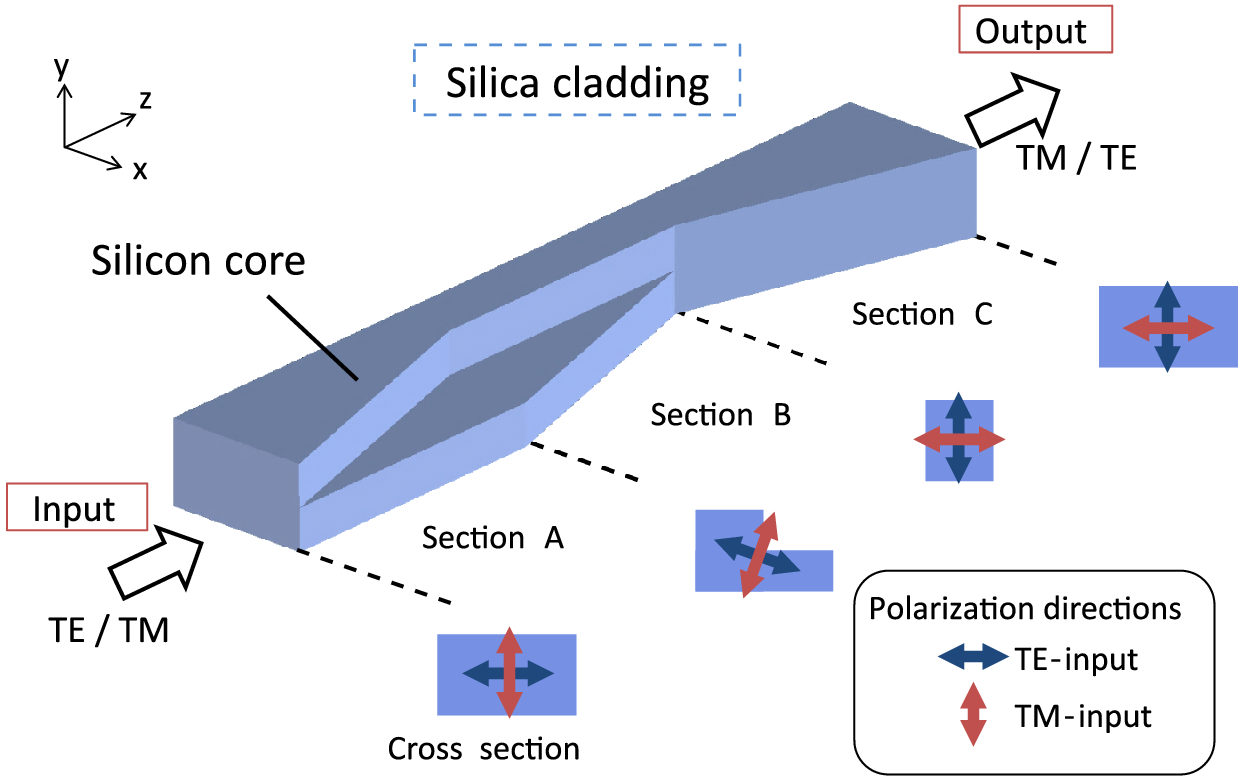
\includegraphics[width=\textwidth]{2-me-1-1}
			\caption{Schematic of the \gls{pr}}
			\label{fig:2_me_1_1}
		\end{subfigure}
		\hfill
		\begin{subfigure}[t]{0.45\textwidth}
			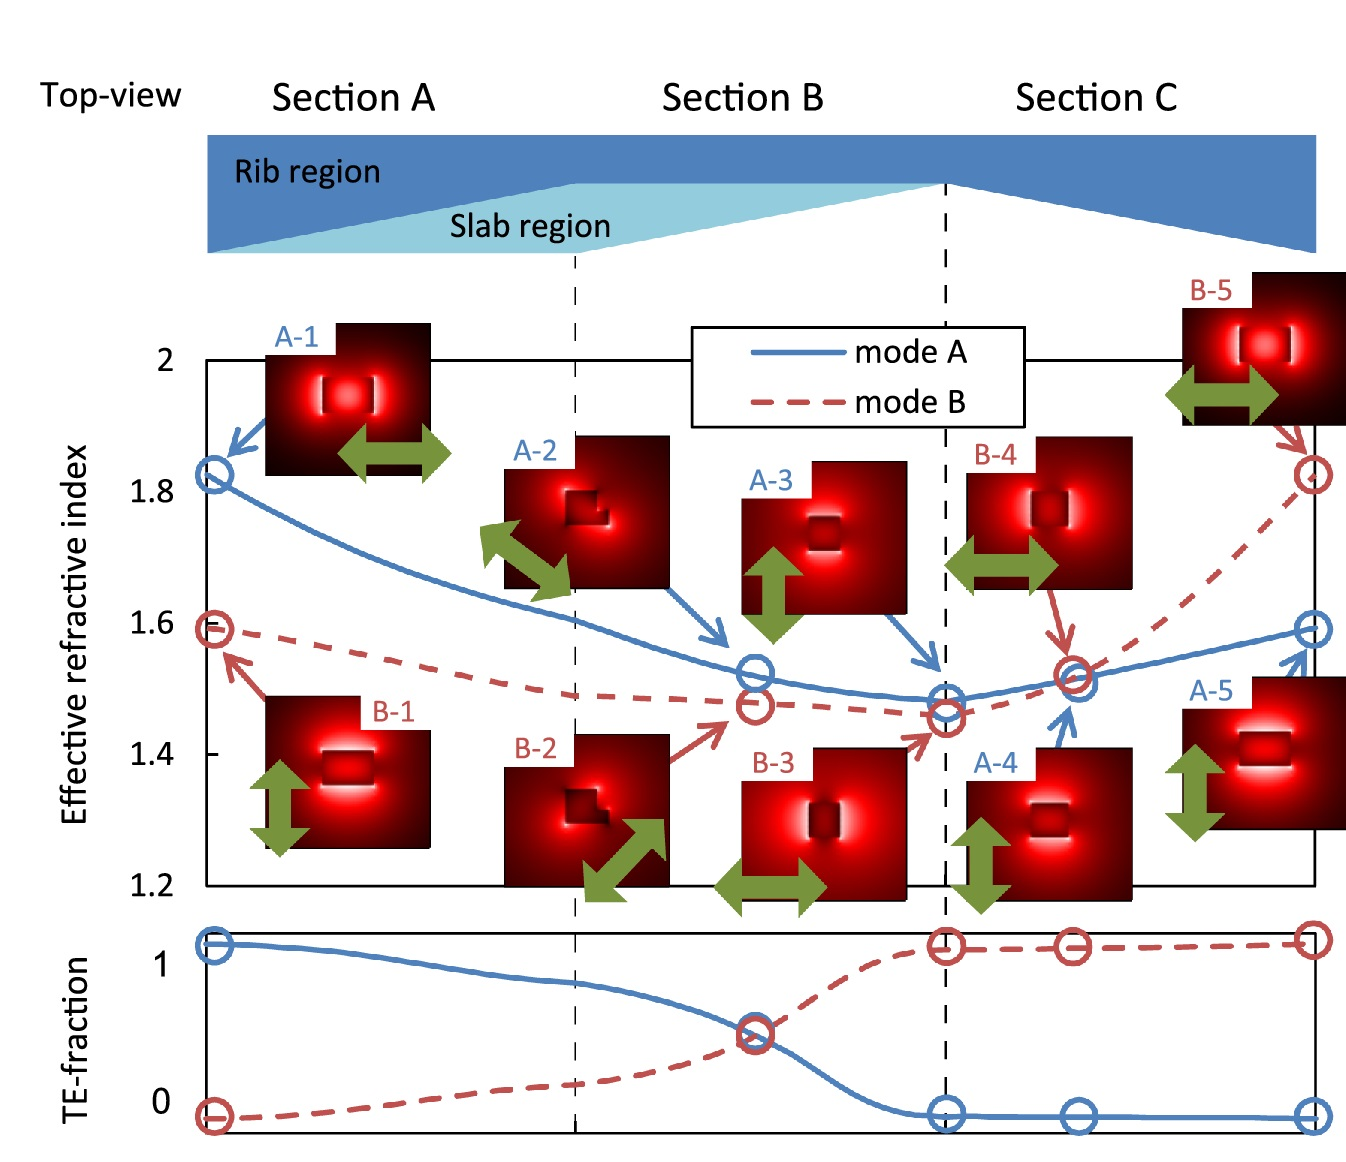
\includegraphics[width=\textwidth]{2-me-1-2}
			\caption{Local mode analysis of the \gls{pr}}
			\label{fig:2_me_1_2}
		\end{subfigure}
		\caption{\gls{pr} using mode evolution, by Goi \textit{et al.} \cite{kazuhiro_integrated_2015}}
	\end{figure}
	\end{minipage}\\\\
	\noindent The \gls{pr} (Fig. \ref{fig:2_me_1_1}) consists of the polarization rotation sections(A and B) with an asymmetric rib waveguide and the mode size conversion section(C) with a nano-tapered waveguide. This design provides both vertical and horizontal asymmetry. \par
	 
	Apart from these, other designs for mode evolution have also been proposed \cite{chen_compact_2011,zhang_efficient_2012,justin_conference_2012}, which has the same basic principle.
	
	\item[$\square$] \textbf{Problem of mode evolution:} In mode evolution, silicon waveguide is specially designed with tapers to enable gradual mode conversion between orthogonal polarization states. This kind of design increases the complexity of fabrication. Also, sharp tips at the end of tapers necessary for low conversion loss are also difficult to make. A pure silicon solution is proposed in \cite{zhang_selected_2010}, but in their structure the input and output silicon waveguides have different thicknesses. The structure in \cite{kazuhiro_integrated_2015} solves this problem at the cost of a longer device length of $230 \si{\micro\meter}$. Efficient design of these kind of \gls{pr}s require trade-off between scattering losses at the tapers versus the device length.
\end{itemize}

			\paragraph*{Mode hybridization:}
Mode hybridization works by abruptly breaking the symmetry of the silicon waveguide cross section. The propagation modes are hybridized due to introduced asymmetry, allowing optical power to be transferred periodically between the two desired polarization states. The propagation modes excite simultaneously the two fundamental hybrid modes of the asymmetric waveguide, which evolve with different propagation constant. The rotation of $90^{\circ}$ is achieved through interference of the two hybridized modes for a length of $L_{\pi}$, according to the principle of wave plates described mathematically, using \ref{eq:jones_matrix_wp3}. 

\begin{itemize}[leftmargin=*]
	
	\item[$\square$] \begin{minipage}[t]{\textwidth}\textbf{Design A: Asymmetric silicon nanowire waveguide as compact \gls{pr}}
	\begin{figure}[H] %h
		\begin{subfigure}[t]{0.45\textwidth}
			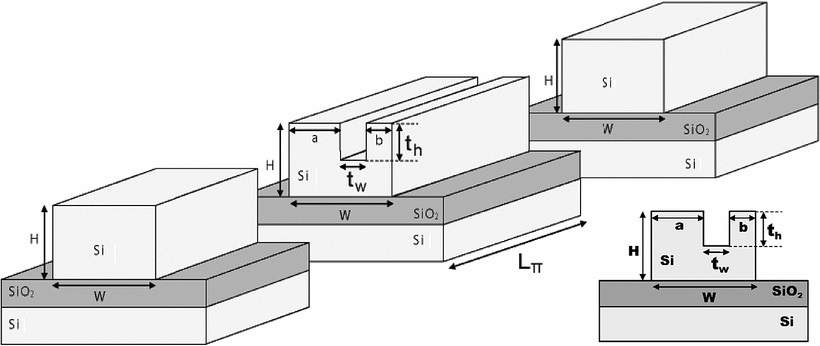
\includegraphics[width=\textwidth]{2-mh-1-1}
			\caption{Schematic diagram of the asymmetric \gls{pr}}
			\label{fig:2_mh_1_1}
		\end{subfigure}
		\hfill
		\begin{subfigure}[t]{0.45\textwidth}
			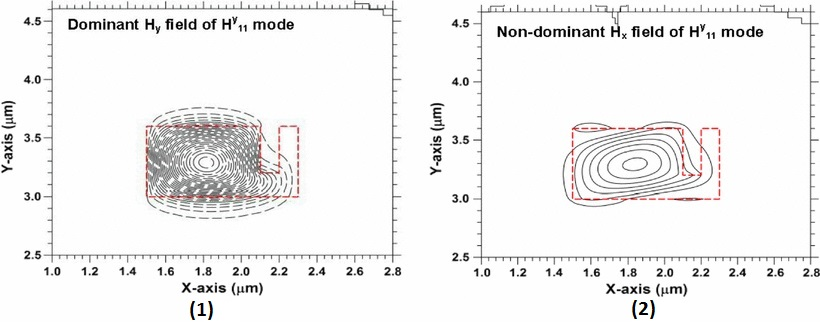
\includegraphics[width=\textwidth]{2-mh-1-2}
			\caption{Contour plots of (1) the dominant $H_y$ field profile and (2) the non-dominant $H_x$ field profile of the $H_{11}^{y}$ mode with $W=800 \si{\nano\meter}$ and $H=800 \si{\nano\meter}$, $t_w=100 \si{\nano\meter}$ and $t_h=400 \si{\nano\meter}$}
			\label{fig:2_mh_1_2}
		\end{subfigure}
		\caption{\gls{pr} using mode hybridization, by Leung \textit{et al.} \cite{leung_numerical_2011}}
	\end{figure}
	\end{minipage}\\\\
	Fig. \ref{fig:2_mh_1_1} depicts the single-stage polarization rotator, which consists of two Si strip waveguides with straight sidewalls, where both are butt coupled to an Si asymmetric strip polarization rotator waveguide in the middle. In the design of a polarization rotator, an asymmetric section which supports the highly hybrid modes is sandwiched between two standard Si waveguides. When a quasi-\gls{te} (or quasi-\gls{tm}) mode from a standard Si waveguide with its polarization angle at nearly zero degrees (or $90^{\circ}$) is launched into the asymmetric section (which supports highly hybrid modes with polarization direction $\pm 45^{\circ }$), then both of them are excited almost equally to satisfy the continuity of the $E_t$ and $H_t$ fields at that interface. These two highly hybrid modes travel along the asymmetric sections. The half-beat length is a key parameter used in order to identify the optimum length of this asymmetrical section to achieve the maximum polarization rotation. The half-beat length is defined as $L_{\pi }= \pi / \Delta \beta$, where $\Delta \beta$ is the difference between the propagation constants of the two hybrid modes. After propagating a distance $L = L_{\pi}$, the original phase condition between the highly polarized modes would be reversed, and the polarization state of the superimposed modes would be rotated by $90^{\circ}$. If a standard Si waveguide (with smaller modal hybridness) is placed at this position, this quasi-\gls{tm} (or quasi-\gls{te}) mode would propagate without any further polarization rotation \cite{leung_numerical_2011}.
	
	\item[$\square$] \textbf{Design B: Efficient silicon \gls{pr} based on mode-hybridization in a double-stair waveguide}\\
	Due to the sudden abruptness introduced in the previous design (Design A) of mode hybridization, the \gls{per} was low. Hence, the abruptness is introduced more gradually in the design, as shown in Fig. \ref{fig:2_mh_2_2}. The design looks like two successive stairs and hence it is called double-stair waveguide. The \gls{pr} \cite{xie_efficient_2015}, based on a double-stair silicon waveguide fabricated with three etch steps as described in Fig.\ref{fig:2_mh_2_1} is better compared to the two-etch-step structure with single-stair cross section \cite{aamer_cmos_2012} because of the higher \gls{per} and broader optical bandwidth achieved. 
	\begin{figure}[H] %h
		\begin{subfigure}[t]{0.45\textwidth}
			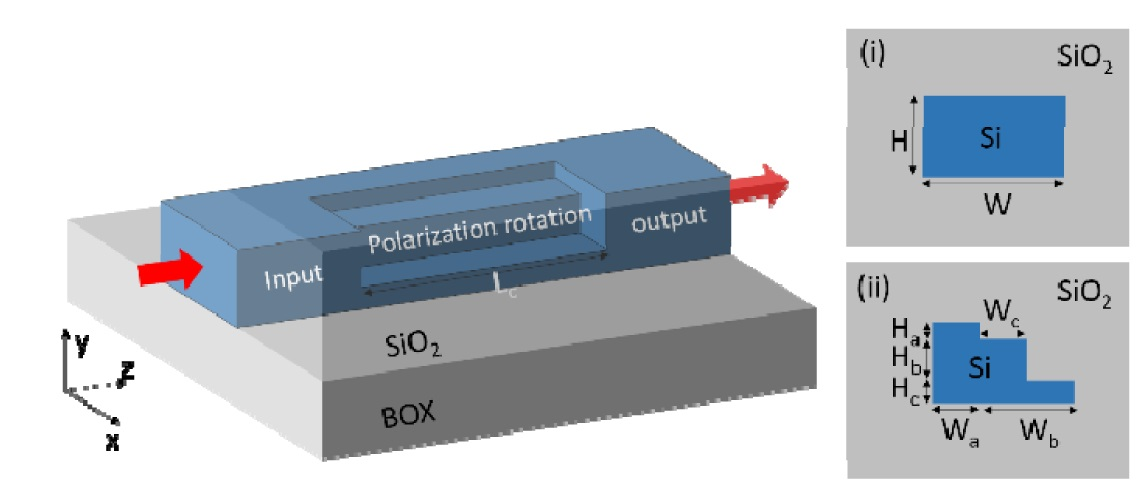
\includegraphics[width=\textwidth]{2-mh-2-1}
			\caption{Schematic structure of the double-stair \gls{pr}. Inset shows the cross-section}
			\label{fig:2_mh_2_1}
		\end{subfigure}
		\hfill
		\begin{subfigure}[t]{0.45\textwidth}
			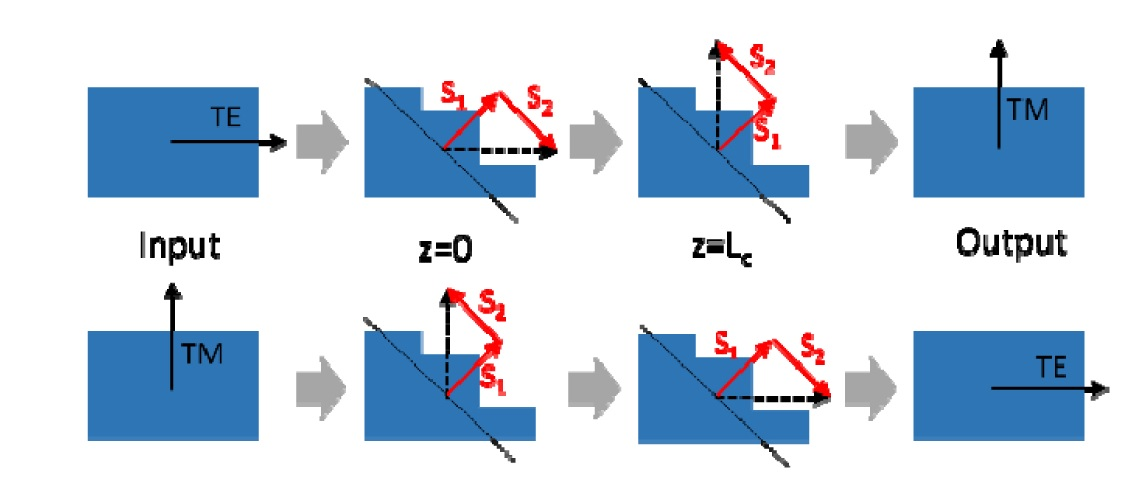
\includegraphics[width=\textwidth]{2-mh-2-2}
			\caption{Polarization rotation process along the waveguide. The arrows indicate the direction of mode electric field. $Z = 0$ is the starting position of the polarization rotation section}
			\label{fig:2_mh_2_2}
		\end{subfigure}
		\caption{\gls{pr} using double-stair waveguide mode hybridization, by Xie \textit{et al.} \cite{xie_efficient_2015}}
	\end{figure}
	\noindent The schematics of the \gls{pr} (Fig. \ref{fig:2_mh_2_1}) consists of the polarization rotation sections and describes the mode conversion along the waveguide.\par
	
	Other designs for mode hybridization have also been proposed \cite{fukuda_integrated_2008,vermeulen_Silicon_2012}, which work on the same principle.
	
	\item[$\square$] \textbf{Problem of mode hybridization:} The narrow trenches ($\sim$\SI{10}{\nano\meter} wide) required for mode hybridization are difficult to pattern and etch with controllable profiles. Recently, a \gls{pr} \cite{aamer_cmos_2012} is realized on a simple strip waveguide by cutting one upper corner of the waveguide in a two-step etch process following the original idea in \cite{wang_ultrasmall_2008}. The pure silicon solution \cite{aamer_cmos_2012}, without the need of extra materials is attractive, but the measured \gls{per} is relatively low around $\sim$\SI{6}{\deci\bel} within a $\sim$\SI{30}{\nano\meter} bandwidth. Although, the double-stair waveguide \cite{xie_efficient_2015}, offers good results but they exhibit wavelength-dependent loss because its working principle relies on interference.
			
\end{itemize}
		
		\subsubsection{Active PR}\label{sec:active_pr}
An active \gls{pr} is generally achieved by multiple tunable controllers which gives a good trade-off between integration and performance. 
	\paragraph*{Tunable PR with thermo-optic effect:} The \gls{pr}s mainly change the \gls{per}, whereas the \gls{tpps} control the polarization phase. The \gls{tpps} are implemented using waveguide heaters placed alongside the waveguide to avoid losses due to interaction of the evanescent field with the metal. The intensity of the waveguide heaters are electrically controlled.	
	
	\begin{itemize}[leftmargin=*]
		
		\item[$\square$]\begin{minipage}[t]{\textwidth}\textbf{Design: Tunable \gls{pr} with phase shifters}
		\begin{figure}[H] %h
			\begin{subfigure}[t]{0.45\textwidth}
				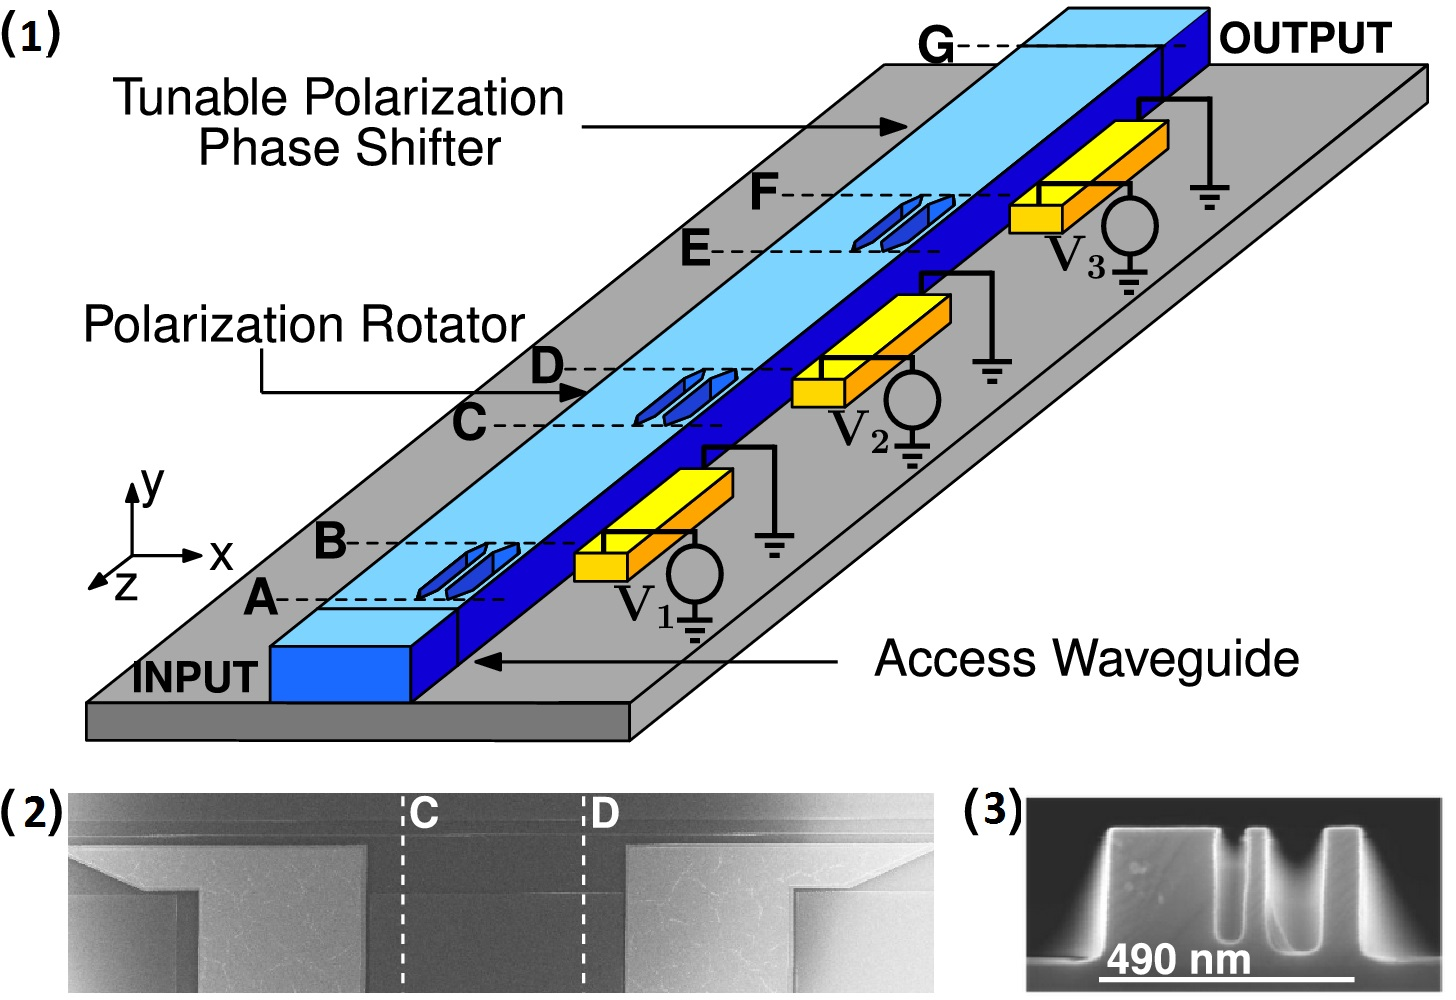
\includegraphics[width=\textwidth]{2-ar-1-1}
				\caption{Schematic of the polarization controller along with the cross section of the \gls{pr}, which uses mode hybridization. The cross section of mode hybridization \gls{pr} can be seen in (3)}
				\label{fig:2_ar_1_1}
			\end{subfigure}
			\hfill
			\begin{subfigure}[t]{0.45\textwidth}
				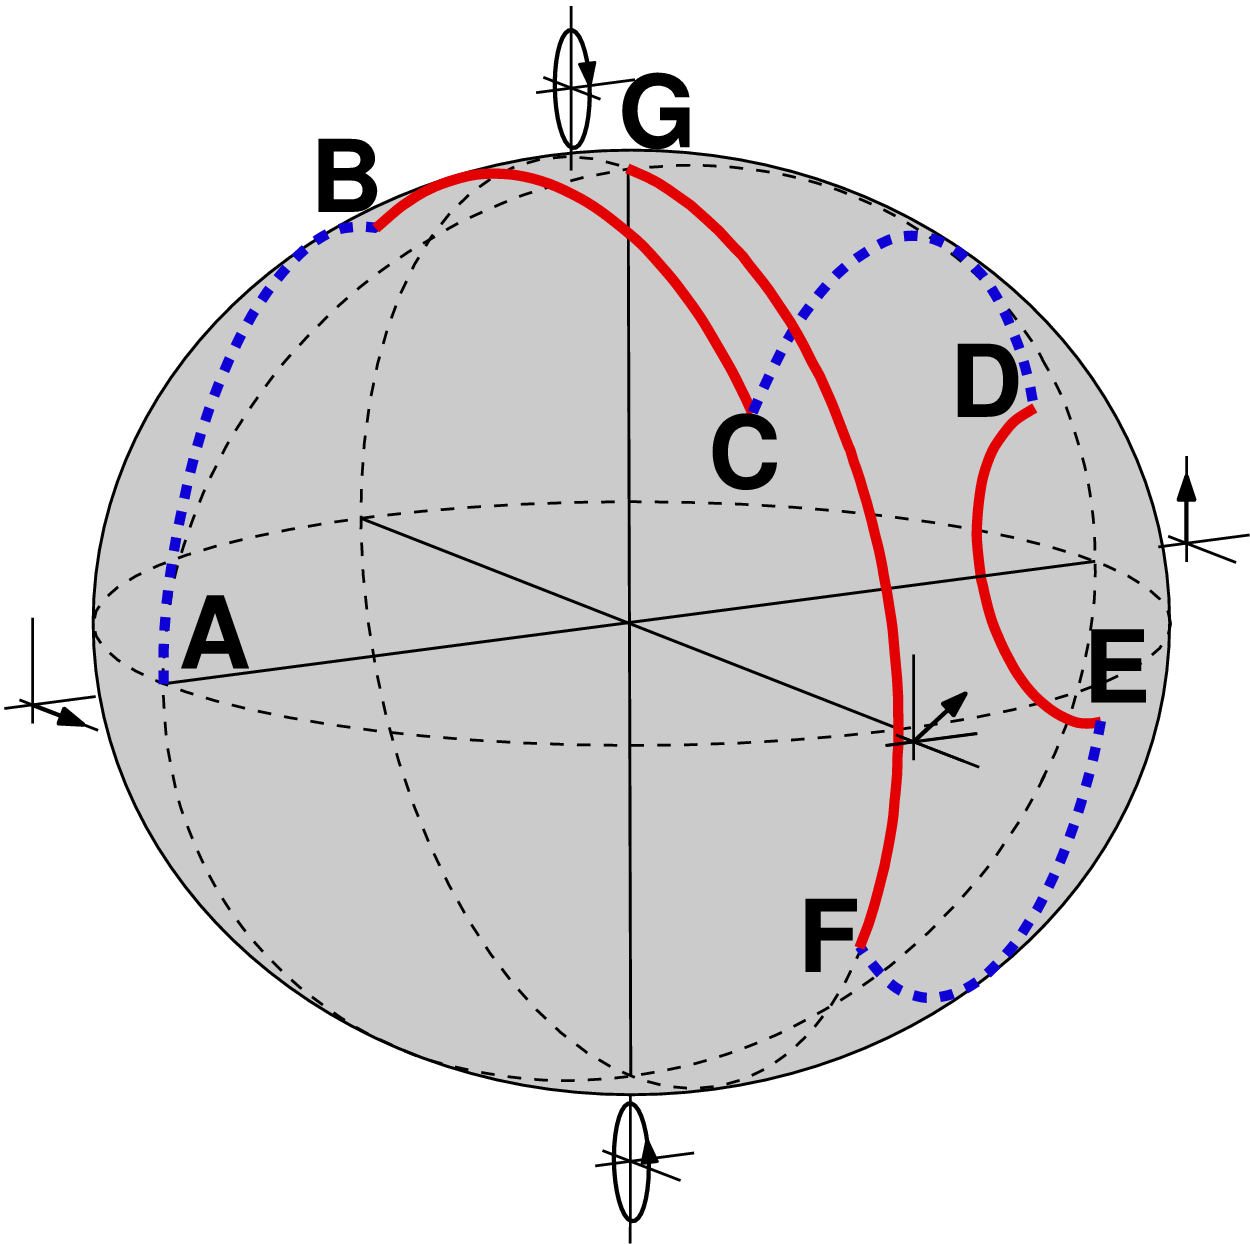
\includegraphics[width=\textwidth]{2-ar-1-2}
				\caption{Evolution of \gls{sop} throughout the device}
				\label{fig:2_ar_1_2}
			\end{subfigure}
			\caption{\gls{pr} control using three \gls{pr} and three \gls{tpps}, by Merenguel \textit{et al.} \cite{sarmiento-merenguel_demonstration_2015}}
		\end{figure}
		\end{minipage}\\\\
		\noindent In the passive \gls{pr}s, the individual \gls{pr} had to produce an exact polarization conversion. This was overcome by the design of the \gls{pr} in Fig. \ref{fig:2_ar_1_1}. The \gls{pr} (Fig. \ref{fig:2_ar_1_1}) consists of three \gls{pr}s and three \gls{tpps} which control the \gls{sop}. The operation of the device is illustrated in Fig. \ref{fig:2_ar_1_2} using the Poincaré sphere \ref{concept:poincare_sphare}. First, a certain \gls{pr} will be performed in the first \gls{pr} (point B). Following the first PR there are two pairs of \gls{tpps}–\gls{pr}. Each \gls{tpps} will tune the polarization phase in order to feed the \gls{pr}s with the suitable polarization phase so that, at the output of the third \gls{pr} (point F), the desired \gls{per} is achieved. The last \gls{tpps} then produces the appropriate polarization phase shift so that the desired \gls{sop} is obtained at the output (point G).
		
		\item[$\square$] \textbf{Drawbacks of PR with thermo-optic effect:}
		Although, the design offers good trade-off between performance and size but still it is limited by the fact that thermal effect can induce phase shift in other waveguides due to cross-talk. This may occur when this system is used in commercial designs with high packing density.
		
		\paragraph*{Tunable PR using Berry's phase:}Berry’s phase is a quantum-mechanical phenomenon that may be observed at the macroscopic optical level through the use of an enormous number of photons in a single coherent state \cite{chiao_manifestations_1986}. In the special case of planar (non-helical) paths, such as the paths typically taken by planar optical waveguides, no significant optical rotation is observed independent of the complexity of the path \cite{tomita_observation_1986}. The key to manifest Berry’s phase in photonic integrated circuits is to introduce out-of-plane three-dimensional waveguides to create a two-dimensional momentum space with non-zero (Gaussian) curvature.
		%\subsubsection{Comparative analysis of available PR}
		
	\end{itemize}
	
	\begin{itemize}[leftmargin=*]
		
		\item[$\square$]\begin{minipage}[t]{\textwidth}\textbf{Design: Tunable \gls{pr} with Berry's phase}
			\begin{figure}[H] %h
				\begin{subfigure}[t]{0.33\textwidth}
					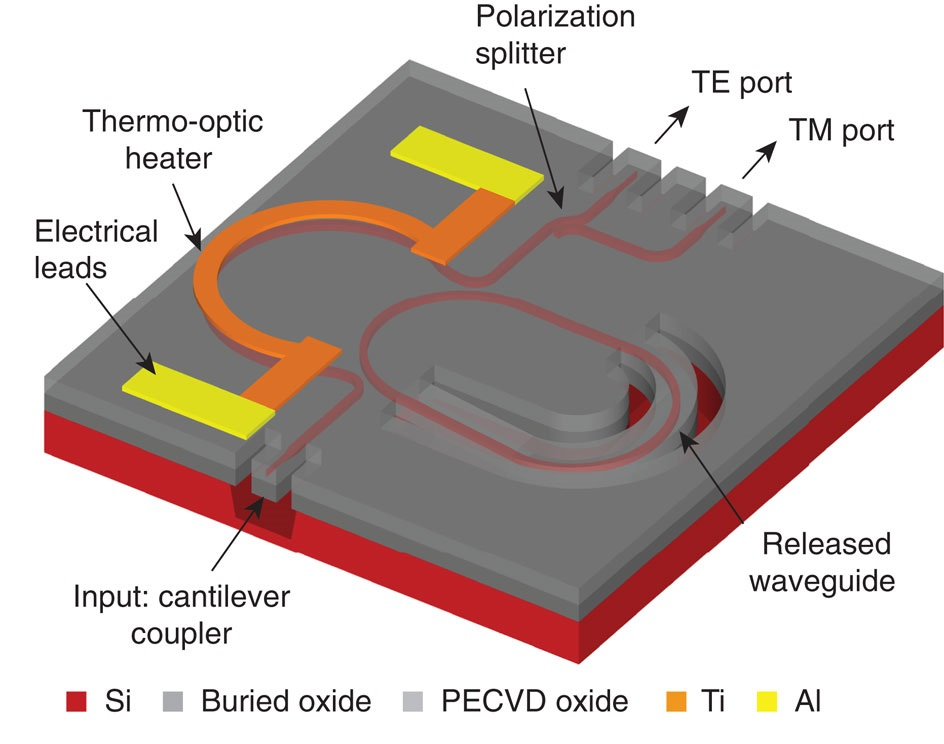
\includegraphics[width=\textwidth]{2-ar-2-1}
					\caption{Schematic of the device}
					\label{fig:2_ar_2_1}
				\end{subfigure}
				\hfill
				\begin{subfigure}[t]{0.33\textwidth}
					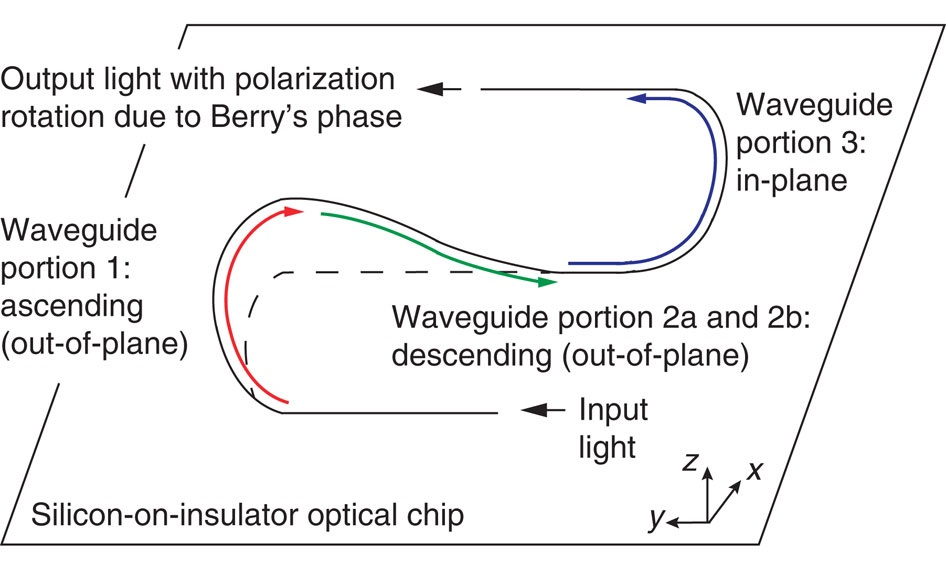
\includegraphics[width=\textwidth]{2-ar-2-2}
					\caption{Layout of device involving out-of-plane waveguides}
					\label{fig:2_ar_2_2}
				\end{subfigure}
				\hfill
				\begin{subfigure}[t]{0.27\textwidth}
					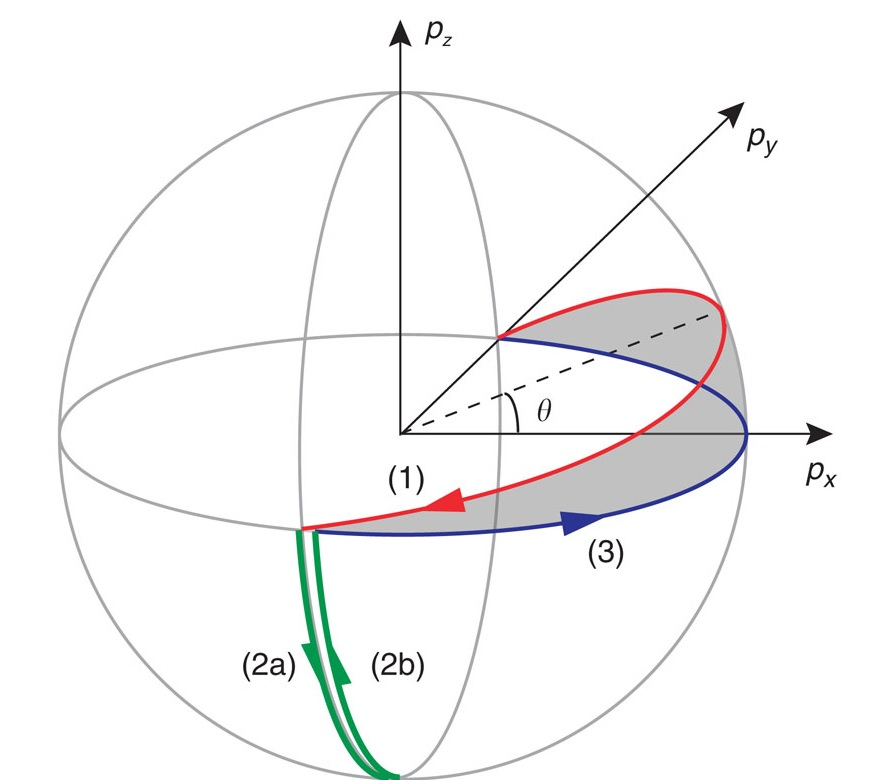
\includegraphics[width=\textwidth]{2-ar-2-3}
					\caption{Evolution of \gls{sop} throughout the device}
					\label{fig:2_ar_2_3}
				\end{subfigure}
				\caption{\gls{pr} control using three \gls{pr} and three \gls{tpps}, by Xu \textit{et al.} \cite{xu_electrically_2014}}
			\end{figure}
		\end{minipage}\\\\
		\noindent Monochromatic light at wavelength $\lambda$ carries a momentum given by $p = p_{x}\widehat {x}+p_{y}\widehat {y}+p_{z}\widehat {z} = \hbar k$, where $k$ is the propagation vector, with magnitude $2\pi/\lambda$ and $\hbar$ is the Planck’s constant divided by $2\pi$. In physical space, the layout consists of three main portions. The first portion, shown in red in Fig. \ref{fig:2_ar_2_2}, consists of an ascending out-of-plane $180^{\circ}$ waveguide bend. The second portion, shown in green, consists of an out-of-plane waveguide that descends to the chip surface. Finally, the third portion consists of an in-plane $180^{\circ}$ bend. In momentum space, the corresponding paths for each waveguide portion are shown in Fig. \ref{fig:2_ar_2_3} using Poincaré sphere (\ref{concept:poincare_sphare}). Light propagation along the three-dimensional path in physical space results in a non-zero subtended solid angle in momentum space, shown as the shaded area in Fig. \ref{fig:2_ar_2_3}. Therefore, the waveguide geometry will exhibit Berry’s phase. A change in wavelength results in a change of the radius of the sphere in momentum space but not the solid angle. If the deflection angle of waveguide portion 1, in the physical space shown in Fig. \ref{fig:2_ar_2_2} is $\theta$, then the output light will appear with polarization rotation equal to $2\theta$ due to Berry’s phase because the magnitude of the solid angle extended by the grey area in momentum space, shown in Fig. \ref{fig:2_ar_2_3}, is $\theta$ \cite{xu_electrically_2014}.
		
		\item[$\square$] \textbf{Drawbacks of PR using Berry's phase:}
		This device uses out-of-plane ring cavity which uses the principles of ring resonator. The ring resonator is limited by its narrow band spectral features which limits bandwidth. Also, the device uses a non-birefringent waveguide, which is lossy in terms of photonic substrate, as an oxide cladding is used to confine light. 	
	\end{itemize}
	\todo{Add FOM}
	%\subsubsection{Comparative analysis of available PR}
\end{document}
